\documentclass[reqno,11pt]{amsart}
\usepackage[letterpaper, margin=1in]{geometry}
\RequirePackage{amsmath,amssymb,amsthm,graphicx,mathrsfs,url,slashed,subcaption}
\RequirePackage[usenames,dvipsnames]{xcolor}
\RequirePackage[colorlinks=true,linkcolor=Red,citecolor=Green]{hyperref}
\RequirePackage{amsxtra}
\usepackage{cancel}
\usepackage{tikz-cd}

% \setlength{\textheight}{9.3in} \setlength{\oddsidemargin}{-0.25in}
% \setlength{\evensidemargin}{-0.25in} \setlength{\textwidth}{7in}
% \setlength{\topmargin}{-0.25in} \setlength{\headheight}{0.18in}
% \setlength{\marginparwidth}{1.0in}
% \setlength{\abovedisplayskip}{0.2in}
% \setlength{\belowdisplayskip}{0.2in}
% \setlength{\parskip}{0.05in}
%\renewcommand{\baselinestretch}{1.05}

\title{Functions of least gradient and minimal laminations}
\author{Aidan Backus}
\date{October 2022}

\newcommand{\NN}{\mathbf{N}}
\newcommand{\ZZ}{\mathbf{Z}}
\newcommand{\QQ}{\mathbf{Q}}
\newcommand{\RR}{\mathbf{R}}
\newcommand{\CC}{\mathbf{C}}
\newcommand{\DD}{\mathbf{D}}
\newcommand{\PP}{\mathbf P}
\newcommand{\MM}{\mathbf M}
\newcommand{\II}{\mathbf I}
\newcommand{\Hyp}{\mathbf H}
\newcommand{\Sph}{\mathbf S}
\newcommand{\Group}{\mathbf G}
\newcommand{\GL}{\mathbf{GL}}
\newcommand{\Orth}{\mathbf{O}}
\newcommand{\SpOrth}{\mathbf{SO}}
\newcommand{\Ball}{\mathbf{B}}

\DeclareMathOperator*{\Expect}{\mathbf E}

\DeclareMathOperator{\avg}{avg}
\DeclareMathOperator{\card}{card}
\DeclareMathOperator{\cent}{center}
\DeclareMathOperator{\ch}{ch}
\DeclareMathOperator{\codim}{codim}
\DeclareMathOperator{\Cyl}{Cyl}
\DeclareMathOperator{\diag}{diag}
\DeclareMathOperator{\diam}{diam}
\DeclareMathOperator{\dom}{dom}
\DeclareMathOperator{\Exc}{Exc}
\newcommand{\ext}{\mathrm{ext}}
\DeclareMathOperator{\Gal}{Gal}
\DeclareMathOperator{\Hom}{Hom}
\DeclareMathOperator{\Iso}{Iso}
\DeclareMathOperator{\Jac}{Jac}
\DeclareMathOperator{\Lip}{Lip}
\DeclareMathOperator{\Met}{Met}
\DeclareMathOperator{\id}{id}
\DeclareMathOperator{\rad}{rad}
\DeclareMathOperator{\rank}{rank}
\DeclareMathOperator{\Rm}{Rm}
\DeclareMathOperator{\Hess}{Hess}
\DeclareMathOperator{\Hol}{Hol}
\DeclareMathOperator{\Prop}{Prop}
\DeclareMathOperator{\Radon}{Radon}
\DeclareMathOperator*{\Res}{Res}
\DeclareMathOperator{\sgn}{sgn}
\DeclareMathOperator{\singsupp}{sing~supp}
\DeclareMathOperator{\Spec}{Spec}
\DeclareMathOperator{\supp}{supp}
\DeclareMathOperator{\Tan}{Tan}
\newcommand{\tr}{\operatorname{tr}}

\newcommand{\Mink}{\mathbf m}
\newcommand{\Ric}{\mathrm{Ric}}
\newcommand{\Riem}{\mathrm{Riem}}
\newcommand*\dif{\mathop{}\!\mathrm{d}}
\newcommand*\Dif{\mathop{}\!\mathrm{D}}
\newcommand{\LapQL}{\Delta^{\mathrm{ql}}}

\newcommand{\dbar}{\overline \partial}

\DeclareMathOperator{\atanh}{atanh}
\DeclareMathOperator{\csch}{csch}
\DeclareMathOperator{\sech}{sech}

\DeclareMathOperator{\Div}{div}
\DeclareMathOperator{\Gram}{Gram}
\DeclareMathOperator{\grad}{grad}
\DeclareMathOperator{\dist}{dist}
\DeclareMathOperator{\spn}{span}
\DeclareMathOperator{\Ell}{Ell}
\DeclareMathOperator{\WF}{WF}

\newcommand{\Two}{\mathrm{I\!I}}

\newcommand{\Lagrange}{\mathscr L}
\newcommand{\DirQL}{\mathscr D^{\mathrm{ql}}}
\newcommand{\DirL}{\mathscr D}

\newcommand{\Hilb}{\mathcal H}
\newcommand{\Homology}{\mathrm H}
\newcommand{\normal}{\mathbf n}
\newcommand{\radial}{\mathbf r}
\newcommand{\evect}{\mathbf e}
\newcommand{\vol}{\mathrm{vol}}

\newcommand{\Bmu}{\boldsymbol \mu}
\newcommand{\Bnu}{\boldsymbol \nu}
\newcommand{\Blambda}{\boldsymbol \lambda}

\newcommand{\pic}{\vspace{30mm}}
\newcommand{\dfn}[1]{\emph{#1}\index{#1}}

\renewcommand{\Re}{\operatorname{Re}}
\renewcommand{\Im}{\operatorname{Im}}

\newcommand{\loc}{\mathrm{loc}}
\newcommand{\cpt}{\mathrm{cpt}}

\def\Japan#1{\left \langle #1 \right \rangle}

\newtheorem{theorem}{Theorem}[section]
\newtheorem{badtheorem}[theorem]{``Theorem"}
\newtheorem{prop}[theorem]{Proposition}
\newtheorem{lemma}[theorem]{Lemma}
\newtheorem{sublemma}[theorem]{Sublemma}
\newtheorem{proposition}[theorem]{Proposition}
\newtheorem{corollary}[theorem]{Corollary}
\newtheorem{conjecture}[theorem]{Conjecture}
\newtheorem{axiom}[theorem]{Axiom}
\newtheorem{assumption}[theorem]{Assumption}

\newtheorem{mainthm}{Theorem}
\renewcommand{\themainthm}{\Alph{mainthm}}

% \newtheorem{claim}{Claim}[theorem]
% \renewcommand{\theclaim}{\thetheorem\Alph{claim}}
\newtheorem*{claim}{Claim}

\theoremstyle{definition}
\newtheorem{definition}[theorem]{Definition}
\newtheorem{remark}[theorem]{Remark}
\newtheorem{example}[theorem]{Example}
\newtheorem{notation}[theorem]{Notation}

\newtheorem{exercise}[theorem]{Discussion topic}
\newtheorem{homework}[theorem]{Homework}
\newtheorem{problem}[theorem]{Problem}

\makeatletter
\newcommand{\proofpart}[2]{%
  \par
  \addvspace{\medskipamount}%
  \noindent\emph{Part #1: #2.}
}
\makeatother



\numberwithin{equation}{section}


% Mean
\def\Xint#1{\mathchoice
{\XXint\displaystyle\textstyle{#1}}%
{\XXint\textstyle\scriptstyle{#1}}%
{\XXint\scriptstyle\scriptscriptstyle{#1}}%
{\XXint\scriptscriptstyle\scriptscriptstyle{#1}}%
\!\int}
\def\XXint#1#2#3{{\setbox0=\hbox{$#1{#2#3}{\int}$ }
\vcenter{\hbox{$#2#3$ }}\kern-.6\wd0}}
\def\ddashint{\Xint=}
\def\dashint{\Xint-}

\usepackage[backend=bibtex,style=numeric]{biblatex}
\renewcommand*{\bibfont}{\normalfont\footnotesize}
\addbibresource{topics.bib}
\renewbibmacro{in:}{}
\DeclareFieldFormat{pages}{#1}


\begin{document}
\begin{abstract}
We show the support of a function of least gradient on a manifold of constant sectional curvature is naturally a minimal lamination.
In the special case that the domain is a hyperbolic surface, this answers some questions of Daskalopoulos--Uhlenbeck.
As an application, we establish some regularity theorems for $1$-harmonic functions.
\end{abstract}

\maketitle

%%%%%%%%%%%%%%%%%%%%%%%%%%%%%%%%%%%%%%%%%%%%%%%%%%%%%%%

% \tableofcontents

\section{Introduction}
Throughout this paper, let $M$ be an oriented Riemannian manifold of metric $g$ and dimension $d$.
For a function $u \in BV_\loc(M)$, we write $\star |\dif u|$ for the total variation of the derivative, c.f. (\ref{total variation}).

\begin{definition}\label{main definitions}
A function $u \in BV_\loc(M)$ has \dfn{least gradient} if for every $v \in BV_\cpt(M)$,
\begin{equation}\label{least gradient functional}
\int_M \star |\dif u| \leq \int_M \star |\dif u + \dif v|.
\end{equation}
A set $U$ of locally finite perimeter has \dfn{least perimeter} if $1_U$ has least gradient.
\end{definition}

Equivalently, a function has least gradient if it is $1$-harmonic \cite{Mazon14}. For a manifold-with-boundary, it is also equivalent to instead allow $v$ to range over trace-free functions \cite[Theorem 2.2]{Sternberg93}.
Functions of least gradient arise naturally in conductivity and magnetic resonance imaging \cite{Tamasan2019, Joy09}, in the numerical analysis of mean curvature flow \cite{Thomas05}, in the continuum-time limit of certain combinatorial games \cite{Kohn06}, and as duals to $\infty$-harmonic functions \cite{daskalopoulos2020transverse}.

Since $\infty$-harmonic functions on hyperbolic surfaces induce geodesic laminations \cite{daskalopoulos2020transverse}, it is natural to conjecture some relationship between functions of least gradient and geodesic laminations.
The goal of this paper is to make this relationship precise.

\begin{definition}
Let $S$ be a closed set.
\begin{enumerate}
\item A (codimension $1$ lamination) \dfn{flow box} for $S$ is a Lipschitz chart in which $S$ can be expressed as $K \times N \subseteq \RR^d$ for some closed $K \subseteq \RR$ and open connected $N \subseteq \RR^{d - 1}$.
\item A (codimension $1$) \dfn{lamination} $\lambda$ in $M$, with support $S$, consists of an atlas of lamination flow boxes whose transition maps preserve the local product structure.
\item A \dfn{leaf} of $\lambda$ is a connected subset of $\supp \lambda = S$ which is locally modeled on the fibers $\{k\} \times N$, $k \in K$.
\item The lamination $\lambda$ is \dfn{minimal} if every leaf of $\lambda$ is $C^2$ and has zero mean curvature.
\end{enumerate}
\end{definition}

See \cite{Morgan88} for a detailed treatment of laminations.
Note carefully that the term ``minimal lamination'' is overloaded: in \cite{daskalopoulos2020transverse,casson_bleiler_1988} it refers to laminations which are minimal with respect to inclusion, which has nothing to do with the condition on leaves.
In the surface case $d = 2$, minimal laminations are also called \dfn{geodesic laminations}, though we will not use this terminology.

\begin{definition}
Let $\lambda$ be a lamination, let $\psi_{ij}$, $i,j \in I$, be the transition maps for $\lambda$, and let $(\chi_i)$ be a partition of unity subordinate to $(\psi_{ij})$.
\begin{enumerate}
\item $\lambda$ is \dfn{measured} if it is equipped with Radon measures $\mu_i$ on each set of leaves $K_i$, $i \in I$, such that $\psi_{ij}^* \mu_i = \mu_j$; in that case we say that $\mu = (\mu_i)$ is a \dfn{transverse measure} to $\lambda$.
\item $\lambda$ is \dfn{oriented} if $\psi_{ij}$ are oriented.
\item If $\lambda$ is a measured oriented lamination, then the \dfn{Ruelle-Sullivan current} $T_\lambda$ of $\lambda$ satisfies, for every $d-1$-form $\varphi$,
$$\int_M T_\lambda \wedge \varphi := \sum_{i \in I} \int_{K_i} \int_{\{k\} \times N_i} \chi_i \varphi \dif \mu_i(k).$$
\end{enumerate}
\end{definition}

Of course, the choice of partition of unity $(\chi_i)$ in the definition of Ruelle-Sullivan current is immaterial.
The Ruelle-Sullivan current is always closed, $\dif T_\lambda = 0$, so it can be locally written $T_\lambda = \dif u$.
The main theorem of this paper characterizes the functions $u$ for which $\dif u$ is a Ruelle-Sullivan current for a minimal lamination:

\begin{mainthm}\label{main thm}
Let $2 \leq d \leq 4$ and suppose that $M$ has constant sectional curvature.
\begin{enumerate}
\item Let $u$ be a function of least gradient.
Then
\begin{enumerate}
\item for every $y \in \RR$, $\partial \{u > y\}$ is either empty or an analytic embedded hypersurface,
\item $\bigcup_{y \in \RR} \partial \{u > y\}$ is the support of a minimal measured oriented lamination $\lambda$ whose leaves are the connected components of the hypersurfaces $\partial \{u > y\}$, and
\item the Ruelle-Sullivan current of $\lambda$ is $\dif u$.
\end{enumerate}
\item Conversely, if $\lambda$ is a minimal measured oriented lamination and $\dif u$ is the Ruelle-Sullivan current of $\lambda$, then $u$ has least gradient.
\end{enumerate}
\end{mainthm}

The r\^ole of the hypothesis $d \leq 4$ is to ensure that the stable Bernstein theorem \cite{Chodosh2021} holds, which ensures that the level sets actually form a lamination.
One can show that the level sets are analytic with the weaker hypothesis $d \leq 7$, and so this result would hold for $d \leq 7$ if we knew a stable Bernstein theorem in that setting.

Moreover, one can remove the assumption that $\dif u$ is exact in the converse statement; a priori, one only knows that the Ruelle-Sullivan current is closed.
Recall that an affine line bundle is \dfn{flat with structure group} $\RR$ if it is equipped with a cover by local trivializations so that the transition maps $\psi_{ij}$ satisfy $\psi_{ij}(v) = v + c_{ij}$ for some constants $c_{ij} \in \RR$.
These transition maps preserve the least-gradient functional so we may discuss sections of such bundles which have locally least gradient.
Any closed current defines such a bundle, as we discuss in \S\ref{LamPrelim}, and one can find a primitive of $\dif u$ in that bundle which has locally least gradient.

Theorem \ref{main thm} was proven by Daskalopoulos--Uhlenbeck in the special case that $M$ is a hyperbolic surface and $u$ is dual to an $\infty$-harmonic function \cite[Theorem 5.2, Theorem 6.10]{daskalopoulos2020transverse}.
In that same paper, Daskalopoulos--Uhlenbeck conjectured that Theorem \ref{main thm} should hold for $M$ a hyperbolic surface, with no duality assumption \cite[Problem 9.4, Conjecture 9.5]{daskalopoulos2020transverse}.

\subsection{Regularity for the one-Laplacian}
Theorem \ref{main thm} strengthens the result of \cite{Mazon14} which gives an Euler-Lagrange characterization of functions of least gradient.
That paper characterized the $1$-harmonic functions in terms of a measurable vector field; we replace this vector field with a Lipschitz vector field.

\begin{corollary}
Let $2 \leq d \leq 4$, suppose that $M$ has constant sectional curvature, and let $u \in BV_\loc(M)$. The following are equivalent:
\begin{enumerate}
\item $u$ has least gradient.
\item There exists a vector field $X \in L^\infty(\star |\dif u|)$ such that $(\dif u, X) = |\dif u|$ and $\Div X = 0$.
\item There exists a locally Lipschitz vector field $X$ such that $(\dif u, X) = |\dif u|$ and $\Div X = 0$.
\end{enumerate}
\end{corollary}
\begin{proof}
By \cite{Mazon14}, the first two conditions are equivalent. TODO: They use existence of the $p$-harmonics to prove this, need to check this for arbitrary manifolds.
Moreover, it is clear that if the last condition holds, then so do the other two.

Finally, if $u$ has least gradient, then Theorem \ref{main thm} we may select oriented Lipschitz coordinates $(x, y) \in \RR^{d - 1} \times \RR$ so that $u(x, y)$ depends on $y$ alone.
Then $\dif y$ is a Lipschitz $1$-form which is conormal to the level sets of $u$, and by gluing together local coordinate patches using a partition of unity and the orientation we may find a Lipschitz conormal $1$-form to the level sets.
Since $\dif u$ is also conormal to the level sets, and the conormal bundle is a line bundle,
$$g^{-1}(\dif y, \dif u) = |\dif y| \cdot |\dif u|.$$
Then $X := ((\dif y)/|\dif y|)^\sharp$ is as desired.
\end{proof}

As a byproduct of the proof of Theorem \ref{main thm}, we also obtain a generalization of G\'orny's regularity theorem \cite[Theorem 1.2]{górny2017planar} for functions of least gradient.
If $E$ is a flat affine line bundle with structure group $\RR$, we write $-E$ for the affine line bundle with transition functions $x \mapsto x - c_{ij}$ where $E$ has transition functions $x \mapsto x + c_{ij}$.

\begin{mainthm}\label{Gorny regularity}
Let $2 \leq d \leq 7$, suppose that $M$ has constant sectional curvature, and let $u: M \to \RR$ have least gradient.
Then:
\begin{enumerate}
\item For every $x \in M$, either $u$ is continuous at $x$ or $u$ has a jump discontinuity along an analytic minimal hypersurface containing $x$, and
\item there exists a flat affine line bundle $E \to M$ with structure group $\RR$ and sections $u_{\text{jmp}}: M \to E$, $u_{\text{cts}}: M \to -E$ of locally least gradient, such that $u_{\text{jmp}}$ has a jump-type derivative, $u_{\text{cts}}$ is continuous, and $u = u_{\text{jmp}} + u_{\text{cts}}$.
\end{enumerate}
\end{mainthm}

This regularity result shows that functions of least gradient are significantly better behaved than general $BV_\loc$ functions.
For example, the function $u(z) = z^{1/2}$ on $\CC$ (with the standard branch) does not admit such a decomposition near $0$ \cite[Example 4.1]{Ambrosio2000FunctionsOB}.

%%%%%%%%%%%%%%

\subsection{Overview of the proof}
Most of the work in the proof of Theorem \ref{main thm} is the following generalization of Miranda's proof \cite{Miranda66} of de Giorgi's regularity theorem \cite{deGiorgi61} for sets of least perimeter to manifolds\footnote{De Giorgi's original paper \cite{deGiorgi61} is notoriously difficulty to find a copy of, as noted by \cite{Miranda66, Giusti77}; moreover, \cite{Miranda66} is in Italian. Therefore, in the proof of Theorem \ref{main lma}, we follow the English-language monograph of Giusti \cite[Part 1]{Giusti77}.}.

\begin{mainthm}[regularity of minimal hypersurfaces]\label{main lma}
Let $2 \leq d \leq 7$ and suppose that $M$ has constant sectional curvature.
Then every set of least perimeter in $M$ is bounded by embedded analytic minimal hypersurfaces.
\end{mainthm}

As in \cite{Miranda66, Giusti77}, we prove Theorem \ref{main lma} by reducing it to a de Giorgi-type lemma, Proposition \ref{de Giorgi}, which controls the oscillation of the conormal $1$-form, or \dfn{excess}, to the reduced boundary to a set of least perimeter.
The key point, as in \cite{Miranda66, Giusti77}, is that the monotonicity formula allows us to approximate a set $U$ of least perimeter by $C^1$ approximate solutions of the minimal surface equation, for which estimates similar to the de Giorgi lemma are well-known.

In the euclidean case, the de Giorgi excess of a set $U$ of least perimeter in an open set $A$ is defined by
$$\Exc_A(U) := |\partial^* U \cap A| - \left|\int_A \partial_\mu 1_U \dif x^\mu \star 1\right|.$$
Here the first term is the surface measure of the reduced boundary of $U$ in $A$, and the integral in the second term is $\RR^d$-valued, using the identification $T_x'\RR^d \cong \RR^d$.
This identification is valid exactly because $\RR^d$ is flat; in particular, the excess is preserved by isometries of $\RR^d$, a key fact in the proof of the de Giorgi lemma.

In \S\ref{excess section} we resolve this conundrum; we sketch the ideas for hyperbolic space $M = \Hyp^d$ for simplicity.
We fix the coordinate frame $(\partial_\mu)$ obtained from the Poincar\'e ball model of hyperbolic geometry; then we push forward $(\partial_\mu)$ by isometries of $M$ to construct coordinate frames $(\partial_\mu^P)$ centered at each point $P \in \Hyp^d$.
We then define the excess
\begin{equation}\label{excess definition prelim}
\Exc_A(U, P) := |\partial^* U \cap A| - \left|\left[\int_A \partial_\mu^P 1_U \star 1\right] \dif x^\mu_P(P)\right|
\end{equation}
which is an element of $T_P' \Hyp^d$.
One can show that $\Exc_A(U, P)$ does not depend on the choice of isometries, but only on the basepoint $P$.

It remains to show that the excess respects translation along geodesics, possibly up to a perturbative term.
Following the strategy of \cite{daskalopoulosPrep1}, we embed $\Hyp^d$ in the Minkowski spacetime $\RR^{1, d}$ as the future unit hyperboloid.
One then obtains the following key estimate (Proposition \ref{translation invariance}): for $P, Q \in A$, $\rho := \diam A$,
$$|\Exc_A(U, P) - \Exc_A(U, Q)| \lesssim \rho^{d + 1}.$$
One can crudely predict this estimate as follows.
Scrutinizing (\ref{excess definition prelim}) we observe that, since we are integrating over the $d-1$-dimensional set $\partial^* U \cap A$, we must estimate the difference of integrands to be $O(\rho^2)$.
On the other hand, the scaling limit $\rho \to 0$ can also be viewed as the nonrelativistic limit, viewing $\Hyp^d$ as the space of positions that a massive particle at the spacetime origin could travel to in one second.
In the nonrelativistic limit, this space converges quadratically fast to the \emph{classical} space of positions a particle could travel to in one second, namely the flat space $\{t = 1\}$.
So the non-translation-invariant tensor fields $\partial_\mu^P$, $\dif x^\mu_P$ converge to coordinate fields on flat space quadratically fast and we conclude the claim.

In \S\ref{Plateau section} we prove the de Giorgi lemma and conclude Theorem \ref{main lma}.
The strategy of the de Giorgi lemma in particular implies that the boundary of a set of least perimeter can be realized as a graph, if it is $C^1$, and so we obtain an embedded (rather than just immersed) hypersurface.

It remains to construct lamination flow boxes; this amounts to showing that the level sets of a function of least gradient have locally uniformly bounded second fundamental forms.
However, since each level set $N$ bounds a set of least perimeter, we can show that $N$ is locally a minimally embedded disk.
Ellipticity of the minimal surface equation implies that $N$ has curvature locally bounded, thus we have a lamination, as we argue in \S\ref{GornySec}.

%%%%%%%%%%%%%%%%%%%%%%%%%%%%%%%%%%%%%%%%%%%%%%%%

\subsection{Acknowledgements}
I would like to thank Georgios Daskalopoulos, Karen Uhlenbeck, Christine Breiner, Chao Li, Trent Lucas, NSF... TODO



%%%%%%%%%%%%%%%%%%%%%%%%%%%%%%%%%%%%%%%%%%%%%%%%%
\section{Preliminaries}\label{Prelims}
\subsection{Notation and conventions}
The operator $\star$ is the Hodge star, thus $\star 1$ is the Riemannian measure.
On a submanifold $\Sigma$ of codimension $\geq 1$, $\vol_\Sigma$ denotes the induced measure and $\star_\Sigma$ denotes the induced Hodge star. We also write $\star_\rho := \star_{\partial B(P, \rho)}$ if $P \in M$ is fixed.

We write $\int_U \omega \wedge \psi$ for the pairing of an $\ell$-current $\omega$ with a compactly supported $\ell$-form $\psi$ in an open set $U$, and identify any $d - \ell$-form $\omega$ with its Poincar\'e dual, the $\ell$-current $\psi \mapsto \int_U \omega \wedge \psi$.

When using the Einstein convention, Greek indices range over $0, 1, \dots$ while Latin indices range over $1, \dots$.
However, even when we have a hyperbolic time $t$ we do \emph{not} sum over it, and do not write $x^0 = t$.
Rather, we write $y := x^0$, which is a spacelike index.
We write $\Japan \xi := \sqrt{1 + |\xi|^2}$ for the Japanese norm of a vector $\xi$.

% We adopt the convention that a manifold is a second-countable and locally euclidean Hausdorff space, and a hypersurface is an embedded (or injectively immersed, if we explicitly specify it) submanifold of codimension $1$.
% We require that any Riemannian metric is $C^\infty$.
% In particular, a manifold may be disconnected, but must be locally connected and with only countably many connected components.

%%%%%%%%%%%%%%%%%%%%%%%%%%%%%%%%%%%%%%%%%%%%%%%
\subsection{Functions of bounded variation}
We identify the derivative of a function $u$ with the $d-1$-current
$$\int_U \dif u \wedge \psi = -\int_U u \dif \psi.$$
For a vector field $X$, we write $\star (Xu) := \dif u \wedge \star (X^\flat)$.
By definition, the space of functions of \dfn{bounded variation} $BV(U)$ is the space of functions $u$ for which
\begin{equation}\label{total variation}
\int_U \star |\dif u| := \sup_{\substack{||\psi||_{C^0} \leq 1\\\supp \psi \Subset U}} \int_U \dif u \wedge \psi
\end{equation}
is finite.
The local finiteness of $\int \star |\dif u|$, and hence the sheaf $BV_\loc$, is diffeomorphism-invariant.

\begin{proposition}[trace theorem and Stokes formula]
Let $U \subseteq M$ be an open set with nonempty Lipschitz boundary, and $u \in BV_\loc(M)$.
Then the trace $v \in L^1_\loc(\partial U)$ is well-defined,
%and is characterized by the conditions that for $\vol_{\partial U}$-almost every $x$,
%\begin{equation}\label{convergence of trace}
%\int_{U \cap B(x, \varepsilon)} \star |v(x) - u| \ll \varepsilon^d,
%\end{equation}
and satisfies for every $d - 1$-form $\psi$,
\begin{equation}\label{Miranda IBP}
\int_U \dif u \wedge \psi + \int_U u \dif \psi = \int_{\partial U} v\psi.
\end{equation}
\end{proposition}
\begin{proof}
By a partition of unity argument we can reduce these results to \cite[Teorema 1]{Miranda67}.
\end{proof}

\begin{proposition}[polar decomposition]
For every $u \in BV_\loc(M)$ there exists a $\star |\dif u|$-measurable section $f$ of the cosphere bundle $S'M$ such that for every compactly supported $d-1$-form $\psi$,
\begin{equation}\label{RNy formula}
\int_M \dif u \wedge \psi = \int_M f|\dif u| \wedge \psi.
\end{equation}
\end{proposition}
\begin{proof}
This follows from \cite[Theorem 4.14]{simon1983GMT}.
\end{proof}

Let $f: M \to S'M$ be given by (\ref{RNy formula}).
As in \cite{Miranda66, Giusti77}, most of the technical work in this paper amounts to controlling the oscillation of $f$ at fine scales.
In order to make this precise, we shall need to take ``averages'' of $f$, but $f$ is a section of a curved vector bundle and so averaging is not well-defined.
We show that it is at least well-defined in the fine-scale limit, by proving a form of the Lebesgue differentiation theorem which is manifestly covariant.

To state our Lebesgue differentiation theorem, observe that if $\omega$ is a current with locally finite total variation $|\omega|$, then for any Riemannian metric, $\star|\omega|$ is a Radon measure, and the sheaves $L^p_\loc(\cdot, \star |\omega|)$, $p \in [1, \infty]$, are independent of the metric.
So we write $L^p_\loc(M, \omega)$ for such a sheaf.
We similarly refer to $\omega$-null sets and $\omega$-measurable sets and functions.

\begin{proposition}[Lebesgue differentiation theorem for a vector bundle]\label{LebesgueDiff}
Let $E \to M$ be a vector bundle over an oriented smooth manifold $M$, $\omega$ a current on $M$ with locally finite total variation $|\omega|$, and $f \in L^1_\loc(M, E, \omega)$.
Then there exists an $\omega$-null set $Z \subset M$ such that for every Riemannian metric on $M$, every trivialization $(F_1, \dots, F_\ell)$ of $E$ with dual trivialization $(F'_1, \dots, F'_\ell)$ of $E'$, and every $P \in M \setminus Z$,
$$f(P) = \lim_{r \to 0} \sum_{i=1}^\ell \left[\frac{\int_{B(P, r)} (F'_i, f) \star |\omega|}{\int_{B(P, r)} \star |\omega|}\right] F_i(P).$$
\end{proposition}

We shall apply this proposition with $E := T'M$, $F_\mu = \dif x^\mu$.
Note carefully that the terms inside the limit \emph{are} dependent on the metric and the choice of trivialization, thus the assertion is that the dependence goes away in the limit, and that the set on which the limit converges is independent.
Indeed, the idea is to scrutinize the proof of the Lebesgue differentiation theorem \cite[Chapter 3, Theorem 1.3]{stein2009real} and observe that the null sets constructed in the proof can be covered by null sets which do not depend on the Riemannian metric or the trivialization.

\begin{proof}
Choose a flat Riemannian metric, let $\dif \mu := \star |\omega|$, $\mathcal F = ((F_i), (F_i'))$ a pair of paralellizations of $E, E'$ such that $(F_i', F_j) = \delta_{ij}$, and $\ell$ the rank of $E$.
Then for every $\delta > 0$ there exists $\tilde f \in C_c(M, E)$ such that $||f - \tilde f||_{L^1(\mu)} < \delta$, thus
\begin{align*}
&\left|\sum_{i=1}^\ell \left[(F_i'(x), f(x)) - \dashint_{B(x, r)} (F_i', f) \dif \mu\right] F_i(x)\right| \\
&\qquad \leq \left|\sum_{i=1}^\ell (F_i'(x), f(x) - \tilde f(x)) F_i(x)\right| + \dashint_{B(x, r)} \left|\sum_{i=1}^\ell (F_i', f - \tilde f)F_i(x) \dif \mu \right| \\
&\qquad \qquad + \left|\sum_{i=1}^\ell \left[(F_i'(x), \tilde f(x)) - \dashint_{B(x, r)} (F_i, \tilde f) \dif \mu\right] F_i(x)\right| \\
&\qquad =: I_1(x) + I_{2, r}(x) + I_{3, r}(x).
\end{align*}
Here the integral defining $I_{2, r}(x)$ is valued in the fiber $E_x$.

By the proof of the Lebesgue differentiation theorem, $\{I_1 > \varepsilon\} \subseteq \{|f - \tilde f| > \varepsilon\}$ and $\{I_{2, r} > \varepsilon\} \subseteq \{\dashint_{B(x, r)} |f - \tilde f|\dif \mu\}$, which are $\mathcal F$-independent sets of measure $\lesssim \delta/\varepsilon$.
Meanwhile $I_{3, r} \to 0$ pointwise as $r \to 0$, so for
\begin{equation}\label{definition of null set}
Z_{\varepsilon, \mathcal F} := \left\{x \in M: \limsup_{r \to 0} \left|\sum_{i=1}^\ell \left[(F_i'(x), f(x)) - \dashint_{B(x, r)} (F_i', f) \dif \mu\right] F_i(x)\right| > 2\varepsilon\right\},
\end{equation}
one has
$$Z_{\varepsilon, \mathcal F} \subseteq \bigcap_{r > 0}\bigcup_{s <r} \{I_{1, s} > \varepsilon\} \cup \{I_{2, s} > \varepsilon\}.$$
The right-hand side is independent of $\mathcal F$ and $\delta$, but has $\mu$-measure $\lesssim \delta/\varepsilon$, so it is $\omega$-null.
Thus the union taken over all possible $\mathcal F$ and $\varepsilon$ is also $\omega$-null.

Now let $g$ be a Riemannian metric and $h$ our flat reference metric.
Then $\varphi := \sqrt{\det g/\det h}$ satisfies $\star_g|\omega| = \varphi \dif \mu$, and as $\varphi$ is continuous it does not contribute in the limit superior in (\ref{definition of null set}).
Moreover, the balls $B_g(x, r)$ have bounded eccentricity with respect to $h$, so we can replace $B(x, r)$ with $B_g(x, r)$ in (\ref{definition of null set}) without affecting $Z_{\varepsilon, \mathcal F}$ \cite[Chapter 3, Corollary 1.7]{stein2009real}.
\end{proof}

\begin{corollary}
The section $f: M \to S'M$ in the polar decomposition (\ref{RNy formula}) satisfies
\begin{equation}\label{Lebesgue point definition}
    f(P) = \left[\lim_{r \to 0} \frac{\int_{B(x, r)} \star \partial_\mu u}{\int_{B(x, r)} \star |\dif u|}\right] ~\dif x^\mu(P)
\end{equation}
for any coordinate system $(x^\mu)$ and any Riemannian metric $g$, and $\star|\dif u|$-almost every $P$.
The exceptional set does not depend on $(x^\mu)$ or $g$.
\end{corollary}

It follows from the above corollary that the following definitions, which a priori refer to the metric or to a choice of coordinate system, are actually completely determined by the smooth structure on $M$.

\begin{definition}
Let $U \subseteq M$. We say that $U$ has \dfn{locally finite perimeter} if $1_U \in BV_\loc(M)$.
In that case we make the following definitions:
\begin{enumerate}
\item The \dfn{measure-theoretic boundary} $\partial U$ is the set of points whose Lebesgue density with respect to $M$ is $\in (0, 1)$.
\item The polar section of $1_U$ is called the \dfn{conormal $1$-form} $\normal_U$ to $\partial U$.
\item The set of points $P$ for which $\normal_U(P)$ exists is the \dfn{reduced boundary} $\partial^* U$.
\item The \dfn{perimeter} $|\partial^* U \cap E|$ in a Borel set $E$ is $\int_E \star |\dif u|$.
\end{enumerate}
\end{definition}

Our definition of reduced boundary and conormal $1$-form follows \cite[Definition 3.3]{Giusti77} and is due to \cite{deGiorgi55}.
See \cite[Chapter 6]{Pugh02} for the definition of Lebesgue density.
Choosing a coordinate system on $M$ in which the volume form is $\dif x^0 \wedge \cdots \wedge \dif x^{d - 1}$, we see from \cite[Chapters 1-4]{Giusti77} that the following properties of the reduced boundary hold:

\begin{proposition}\label{locality of Caccioppoli}
    Let $U$ be a set of locally finite perimeter.
    Then:
    \begin{enumerate}
    \item $\partial^* U$ is either empty or $d-1$-dimensional in the Hausdorff sense, and is $d-1$-rectifiable.
    \item $\partial^* U$ is a dense subset of $\partial U$.
    \item If $\normal_U$ extends to a continuous $1$-form on $\partial U$, then $\partial^* U = \partial U$ is a $C^1$ embedded hypersurface.
    \item If $\partial^* U = \partial U$ is a $C^1$ hypersurface, then $\normal$ is the conormal $1$-form on $\partial U$ as defined in differential topology, and $\star |\dif 1_U|$ is the induced measure on $\partial U$.
\end{enumerate}
\end{proposition}

As a first application of Proposition \ref{locality of Caccioppoli} we recover the following formulation of the coarea formula.

\begin{proposition}[coarea formula]\label{Coarea2}
Let $u \in BV_\loc(M)$ and $E$ an open set. Then
\begin{equation}\label{coarea formula}
\int_E \star |\dif u| = \int_{-\infty}^\infty |E \cap \partial^* \{u > y\}| \dif y.
\end{equation}
\end{proposition}
\begin{proof}
Reasoning identically to \cite[Theorem 1.23]{Giusti77}, we may assume that $u \in C^\infty(M)$.
If this is true and also $u$ has no critical points, then (\ref{coarea formula}) follows from Fubini's theorem, the fact that $|E \cap \partial \{u > y\}|$ is the surface area of $E \cap \{u = y\}$ (by Proposition \ref{locality of Caccioppoli}), and the change-of-variables formula.
However the left-hand side of (\ref{coarea formula}) is unaffected by critical points of $u$, and the right-hand side of (\ref{coarea formula}) is unaffected by critical values of $u$ by Sard's theorem, so (\ref{coarea formula}) holds even if $u \in C^\infty(M)$ has critical points.
% Taking a sequence in $C^\infty(M)$ that converges to $u$ in $L^1_\loc(M)$\footnote{Recall that $C^\infty(M)$ is not dense in $BV_\loc(M)$.}, and applying Fatou's lemma and the semicontinuity of total variation, we conclude the $\geq$ direction of (\ref{coarea formula}).
% Moreover, Stokes' theorem gives that for every $d-1$-form $\psi$ such that $||\psi||_{L^\infty} \leq 1$ and $\supp \psi \Subset E$,
% $$\int_E u \wedge \dif \psi = \int_{-\infty}^\infty \int_E |\psi| \star |\dif 1_{\partial \{u > y\}}| \dif y \leq \int_{-\infty}^\infty |E \cap \partial \{u > y\}| \dif y.$$
% Taking the supremum over $\psi$ we obtain the direction $\leq$ in (\ref{coarea formula}).
\end{proof}

%%%%%%%%%%%%%%%%%%%%%%%
\subsection{Functions of least gradient}
We write
$$\eta(u, U) := \inf_{v \in BV_\cpt(U)} \int_U \star |\dif(u + v)|$$
for $u \in BV_\loc(M)$ and $U \subseteq M$ open with Lipschitz boundary, thus $u$ has least gradient iff $\eta(u, U) = \int_U \star |\dif u|$ for every $U$.
Reasoning identically to \cite[Lemma 5.6]{Giusti77}, we have the following a priori estimates:

\begin{proposition}[a priori estimates]
For any functions $u, v \in BV(U)$,
\begin{align}
|\eta(u, U) - \eta(v, U)| &\leq ||u - v||_{L^1(\partial U)} \label{a priori estimate 1} \\
\eta(u, U) &\leq ||u||_{L^1(\partial U)} \leq |\partial U| \cdot ||u||_{L^\infty(M)}. \label{a priori estimate 2}
\end{align}
\end{proposition}

\begin{definition}
A sequence $(u_n)$ in $BV_\loc(M)$ (not necessarily of the same trace) has \dfn{approximately least gradient} if for every open $U \subseteq M$ with Lipschitz boundary,
$$\limsup_{n \to \infty} \int_U \star |\dif u_n| \leq \liminf_{n \to \infty} \eta(u_n, U) < \infty.$$
\end{definition}

\begin{proposition}[Miranda stability theorem]\label{Miranda convergence}
If a sequence of functions $(u_n)$ has approximately least gradient and $u_n \to u$ in $L^1_\loc(M)$, then $u$ has least gradient, and for every open set $U \Subset M$ with Lipschitz boundary such that $\int_{\partial U} \star |\dif u| = 0$, one has
\begin{equation}\label{convergence in total variation}
\lim_{n \to \infty} \int_U \star |\dif u_n| = \int_U \star |\dif u|.
\end{equation}
\end{proposition}
\begin{proof}
The proof is similar to Teorema 3 and Osservazione 3 in \cite{Miranda67}; we just note the necessary modifications.
Suitable generalizations of Teorema 2 and Osservazione 2 follow from the Stokes formula.
One needs to add a term of size $o(1)$ to the right-hand side of the inequalities (2.8), (2.9), (2.13), and (2.14); however, in the limit, this term vanishes and so the conclusions (2.15) and (2.16) are unaffected.
\end{proof}

The somewhat unusual condition $\int_{\partial U} \star |\dif u| = 0$ refers to the same Radon measure $\star |\dif u|$ that acts on the open sets of $M$, not on a measure that acts on the relatively open subsets of $\partial U$.
It should be interpreted as a transversality condition: if $u$ is the indicator function of a set $Z$ with $C^\infty$ boundary, then $\int_{\partial U} \star |\dif u| = 0$ if $\partial U$ is transverse to $\partial Z$.
In particular, the notion of convergence in the Miranda stability theorem is weaker than convergence in $BV_\loc(M)$.
From the Miranda stability theorem and the compactness of the natural map $BV_\loc(M) \to L^1_\loc(M)$ we conclude:

\begin{corollary}\label{compactness}
Every sequence $(u_n)$ of approximately least gradient which is bounded in $L^1_\loc(M)$ converges in $L^1_\loc(M)$ and almost everywhere along a subsequence to a function of least gradient $u$ such that for every open set $U \Subset M$ of Lipschitz boundary such that $\int_{\partial U} \star |\dif u| = 0$, one has (\ref{convergence in total variation}).
\end{corollary}

\begin{definition}
For a function $u$ on $M$, $P \in M$ we define the \dfn{tangent rescaling} of $u$ at $P$ to be the net of functions $u_t: T_PM \to \RR$, given by
$$u_t(v) = u\left(\exp_P(tv)\right).$$
\end{definition}

\begin{proposition}\label{blowup theorem}
Suppose that $U$ is an open set with least perimeter in $B(P, r)$, $P \in \partial^* U$, and $u = 1_U$.
Furthermore, suppose that $d \leq 7$.
Then the tangent rescaling of $u$ converges as $t \to 0$ along a subsequence (that we also denote $t \to 0$) in $L^1_\loc$ and almost everywhere, to the indicator function $v$ of a half-space $C \subset T_PM$ such that $0 \in \partial C$.
Moreover, for every open set $V \Subset T_PM$ of Lipschitz boundary such that $\partial V$ is transverse to $\partial C$,
$$\lim_{t \to 0} \int_V \star |\dif u_t| = \int_V \star |\dif v|.$$
\end{proposition}
\begin{proof}
We first observe that the tangent rescaling $(u_t)$ has approximately least gradient in $T_PM$ (where we give $T_PM$ its euclidean metric).
This follows from the Taylor expansion of the Riemannian measure and reasoning as in the proof of \cite[Theorem 9.3]{Giusti77}, and so by Corollary \ref{compactness}, there exists a set $C$ of least perimeter in $T_PM$, such that the tangent rescaling converges to $v := 1_C$ in the desired sense.
But $T_PM$ is isometric to $\RR^d$, $d \leq 7$, so by the Bernstein--Fleming theorem \cite[Theorem 17.3]{Giusti77}, $\partial C$ is a hyperplane.
The fact that $0 \in \partial C$ follows from the fact that $P \in \partial^* U$.
% To prove the claim, write $|\cdot|'$, $\star'$ for the notions taken in the tangent space with its euclidean geometry, and write $U_t$ for the set indicated by $u_t$.
% If $V$ is a precompact open subset of $T_PM$, $V_t = \{v \in T_PM: tv \in V\}$, then we have the scale-invariance
% \begin{equation}\label{almost blowup scale invariance}
% |\partial^* U_t \cap V|' = t^{1 - d}|\partial^* U_1 \cap V_{1/t}|'.
% \end{equation}
% From (\ref{almost blowup scale invariance}) and the Taylor expansion (\ref{expand volume form}),
% $$t^{d - 1} |\partial^* U_t \cap V|' = |\partial^* U_1 \cap V_{1/t}|' \leq e^{O(t^2)} |\partial^* U \cap \exp_P(V_{1/t})|.$$
% For every $w \in BV_\cpt(V)$, the least-gradient nature of $u$ gives
% $$|\partial^* U \cap \exp_P(V_{1/t})| \leq \int_{(\exp_P)_* V_{1/t}} \star |\dif(u + (\exp_P)_* w_{1/t})| \leq e^{O(t^2)} \int_{V_{1/t}} \star'|\dif(u_1 + w_{1/t})|'.$$
% Therefore, after applying (\ref{almost blowup scale invariance}) and (\ref{expand volume form}) again,
% $$|\partial^* U_t \cap V|' \leq e^{O(t^2)} t^{1 - d} \int_{V_{1/t}} \star' |\dif (u_1 + w_{1/t})| = e^{O(t^2)} \int_V \star' |\dif (u_t + w)|.$$
% Since $V,w$ were arbitrary, we conclude that $(u_t)$ has approximately least gradient.
\end{proof}


%%%%%%%%%%%%%%%%%%%%%%%%%%%%%%%%%%%%%%%%%%%%%%
\section{Averages of differential forms}\label{excess section}
\subsection{Construction of averages}
The classical de Giorgi lemma is concerned with the rate of convergence in the Lebesgue differentiation theorem of the conormal $1$-form $\normal_U$ to a set $U$ of least perimeter.
As with most tools of harmonic analysis, the Lebesgue differentiation theorem breaks diffeomorphism symmetry.
This is true even when stated carefully as in Proposition \ref{LebesgueDiff}, which asserts that the limiting behavior is diffeomorphism-invariant, but \emph{not} that the rate of convergence of the averages is.

The issue is that, if the Levi-Civita connection $\nabla$ is flat, then $\nabla$ induces canonical isomorphisms $T_P'M \to T_Q'M$ for each $Q$ close to $P$ that we can ignore the effects of monodromy.
Hence $\nabla$ identifies $1$-forms $\xi$ defined near $P$ with $T_P'M$-valued functions $\tilde \xi$.
One can then define the average of $\xi$ with respect to a measure $\omega$,
\begin{equation}\label{averages and flat connections}
\avg_U \xi := \dashint_U \tilde \xi \dif \omega
\end{equation}
where the right-hand side is a vector-valued integral and $U \ni P$, and so $\avg_U \xi \in T_P'M$ (but could also be viewed as a $1$-form by parallel translation).
In particular, the choice of $P$ does not matter; in other words this notion of averaging respects translation and rotation symmetries.
This fails, however, if $\nabla$ has curvature, even if it arises from a metric $g$ with translation and rotation symmetries: the issue is that the holonomy group of $\nabla$ obstructs the naturality of the isomorphisms $T_P'M \to T_Q'M$.

Now suppose that $\nabla$ is the Levi-Civita connection of a metric $g$ with constant sectional curvature, thus $g$ has translation and rotation symmetries.
Then $\nabla$ still has holonomy, but we can define averages still, as follows.

If $g$ has constant sectional curvature $K \in \RR$, then we can cover $M$ by charts $(x^\mu)$ in which $g$ takes the form
\begin{equation}\label{constant sectional curvature metric}
g_{\mu\nu} = \frac{\delta_{\mu\nu}}{(1 + K|x|^2/4)^2}.
\end{equation}
Without loss of generality, $M$ is equal to such a chart.
We fix the origin $O$, where $x = 0$, and introduce a smooth family $(\Phi^P)_{P \in M}$ of oriented isometries $M \to M$, such that $\Phi^O$ is a rotation and $\Phi^P(O) = P$.
We write
$$\partial^P_\mu := \Phi^P_* \partial_{x^\mu}$$
and $x^\mu_P := x^\mu \circ \Phi^P$.
The choices of $(x^\mu)$ and $(\Phi^P)$ amount to selecting an oriented coordinate frame based at $P$ in which the metric takes the form (\ref{constant sectional curvature metric}).
The family of frames $(\partial^P_\mu)$ is uniquely determined up to a \dfn{gauge transformation}, that is, a section $\chi$ of the bundle $\SpOrth(TM) \to M$.

\begin{definition}
The \dfn{average} of a $1$-form $\xi$ over an open set $U$ based at $P$ with respect to a measure $\omega$ to be
$$\avg_{U, P, \omega} \xi := \left[\dashint_U (\xi, \partial^P_\mu) \dif \omega\right] \dif x^\mu(P).$$
\end{definition}

We sometimes suppress the subscripts $U, P, \omega$ if they are clear or irrelevant.
By definition, $\avg_{U, P} \xi$ is again an element of $T_P'M$, and one can check that if $K = 0$ then it equals (\ref{averages and flat connections}).
Proposition \ref{LebesgueDiff} implies that $\avg_{B(P, r), P} \xi$ converges to $\xi(P)$ as $r \to 0$ unless $P$ is an element of an $\omega$-null set.
It is also gauge invariant (or equivalently rotation invariant): if we obtain $\widetilde{\avg_{U, P}} \xi$ from a coordinate system obtained by rotating $\Phi^P$ by $\chi(P) \in \SpOrth(T_PM)$, then
$$\widetilde{\avg_{U, P, \omega}} \xi = \left[\dashint_{B(P, r)} \chi^\nu_\mu \xi_\nu \dif \omega\right] (\chi(P)^{-1})_\lambda^\mu \dif x^\lambda_P(P) = \avg_{U, P} \xi.$$
The average also satisfies the following sort of weak translation-invariance:

\begin{proposition}\label{translation invariance}
The average in an open set $A$ satisfies
$$||\avg_{A, P} \xi| - |\avg_{A, Q} \xi|| \lesssim (\diam A)^2 ||\xi||_{C^0}.$$
\end{proposition}

In the proof of Proposition \ref{translation invariance}, we will fill in the details in the case $K < 0$, as the case $K = 0$ is trivial and the case $K > 0$ is similar and strictly easier; we shall briefly remark on that later.

We first rapidly review the facts about the hyperboloid model that we will need.
For a more thorough discussion which uses many of the same ideas as the proof of Proposition \ref{translation invariance}, see \cite[\S3.1, \S4.1]{daskalopoulosPrep1}.
Let $\RR^{1, d} = \RR_t \times \RR_y \times \RR_x^{d - 1}$ be the Minkowski spacetime with its metric $-\dif t^2 + \dif y^2 + |\dif x|^2$.
Expressing $\Hyp^d$ in the Poincar\'e ball model, we obtain an embedding
\begin{align*}
\Psi: \Hyp^d &\to \RR^{1, d} \\
x &\mapsto \frac{1}{1 - |x|^2/4 - y^2/4} \begin{bmatrix}1 + |x|^2/4 + y^2/4\\y \\ x\end{bmatrix}
\end{align*}
whose image is the unit future hyperboloid, as in the proof of \cite[Proposition 3.5]{lee1997riemannian}, and $\Psi(O) = (1, 0, 0)$.
This embedding induces a split exact sequence of $\SpOrth^+(\RR^{1, d})$-bundles over $\Hyp^d$
\begin{equation}\label{splitting of tangent bundle}
0 \to T\Hyp^d \to \Hyp^d \times \RR^{1, d} \to N\Hyp^d \to 0
\end{equation}
where $N\Hyp^d$ is the normal bundle of the embedding $\Psi$ \cite[(3.4)]{daskalopoulosPrep1}.
Here $\SpOrth^+(\RR^{1, d})$ is the properly orthochronous Lorentz group.

\begin{lemma}
The splitting (\ref{splitting of tangent bundle}) induces canonical isomorphisms of $\SpOrth^+(\RR^{1, d})$-representations
\begin{equation}\label{SES}
\RR^{1, d} = N'_P \Hyp^d \oplus T'_P \Hyp^d.
\end{equation}
for each $P \in \Hyp^d$.
Writing $\xi_O$ for the orthogonal projection of $\xi \in T'_P \Hyp^d \subseteq \RR^{1, d}$ to $T'_O \Hyp^d$,
\begin{equation}\label{Dask estimate}
|\xi| \leq |\xi_O| \leq e^{\dist(O, P)^2/2} |\xi|.
\end{equation}
\end{lemma}
\begin{proof}
We consider the adjoint sequence
$$0 \to N' \Hyp^d \to \Hyp^d \times \RR^{1, d} \to T' \Hyp^d \to 0$$
to (\ref{splitting of tangent bundle}).
Since (\ref{splitting of tangent bundle}) is split exact, we have a direct sum of $\SpOrth^+(\RR^{1, d})$-bundles $\Hyp^d \times \RR^{1, d} = T' \Hyp^d \oplus N' \Hyp^d$.
Here $\Hyp^d \times \RR^{1, d}$ is equipped with its trivial connection $\dif$ and has trivial monodromy group, so the parallel transport maps induce canonical isomorphisms between each fiber of $\Hyp^d \times \RR^{1, d}$ and $\RR^{1, d}$.
Therefore we have canonical isomorphisms (\ref{SES}).

Now (\ref{Dask estimate}) easily follows from \cite[\S4.1]{daskalopoulosPrep1}:\footnote{One may object that \cite[\S4.1]{daskalopoulosPrep1} refers to the splitting of the tangent bundle (\ref{splitting of tangent bundle}) rather than the cotangent bundle, but after conjugating by a musical isomorphism we see that the same estimates hold for the splitting of the cotangent bundle.}
By (\cite[(4.1)]{daskalopoulosPrep1}), $\xi_O$ is just $\xi$ with its timelike part $\xi_t$ set to $0$, thus
$$|\xi_O|^2 = |\xi_x|^2 + |\xi_y|^2 \geq |\xi_x|^2 + |\xi_y|^2 - |\xi_t|^2 = |\xi|^2.$$
On the other hand, by \cite[Lemma 4.2, Lemma 4.1]{daskalopoulosPrep1},
\begin{align*}
|\xi_O| &\leq (1 + |P - O|^2/2) |\xi| \leq (1 + \rho^2 \cosh \rho/2) |\xi| \leq e^{\rho^2/2} |\xi|. \qedhere
\end{align*}
\end{proof}

\begin{lemma}
The pushforward morphism $\Psi_*: T_{(x, y)} \Hyp^d \to T_{\Psi(x, y)} \RR^{1, d}$ is
\begin{equation}\label{pushforward estimates}
\Psi_* = \begin{bmatrix}y & x \\ 1 \\ & \id \end{bmatrix} + O(|x|^2 + y^2).
\end{equation}
\end{lemma}
\begin{proof}
We compute for $f(y, x) := |x|^2/4 + y^2/4$ that
\begin{align*}
\Psi_* &= \frac{1}{1 - f} \begin{bmatrix} \partial_y f & \partial_x f \\ 1 \\ & \id \end{bmatrix} + \frac{1}{(1 - f)^2} \begin{bmatrix}(1 + f) \partial_y f & (1 + f) \partial_x f \\
y \partial_y f & y \partial_x f \\
(\partial_y f) x & x \otimes \partial_x f
\end{bmatrix} \\
&= \begin{bmatrix}y & x \\ 1 \\ & \id \end{bmatrix} + O(|x|^2 + y^2)
\end{align*}
since $f(y, x) = O(|x|^2 + y^2)$ and $2\dif f(y, x) = (y, x)$.
\end{proof}

\begin{lemma}
Let $P \in \Hyp^d$ be given by $x^i = 0$, $y = \rho$. Consider the Lorentz boost
$$\Lambda := \begin{bmatrix}\cosh \rho & \sinh \rho \\ \sinh \rho & \cosh \rho \\ &&\id\end{bmatrix}$$
Up to a gauge transformation, it holds that for each $X \in \Hyp^d$, $Y := (\Phi^P)^{-1}(X)$, the below diagram commutes:
\begin{equation}\label{Lorentz boost diagram}
\begin{tikzcd}[column sep=50pt, row sep=30pt]
\RR^{1, d} \arrow[r, "\Lambda"] & \RR^{1, d} \\
T_Y \Hyp^d \arrow[u, "\dif \Psi(Y)"] \arrow[r, "\dif \Phi^P(Y)"] & T_X \Hyp^d \arrow[u, "\dif \Psi(X)"]
\end{tikzcd}
\end{equation}
\end{lemma}
\begin{proof}
Up to a gauge transformation, we may assume that $\Phi^P$ acts by hyperbolic translation along the $y$-axis.
On the other hand, $\Lambda \in \SpOrth^+(\RR^{1, d})$, so it preserves the unit future hyperboloid $\Psi(\Hyp^d)$ and acts by isometry.
Since $\Lambda$ clearly also preserves $\{(t, y, 0) \in \RR^{1, d}\}$, $\Lambda|\Psi(\Hyp^d)$ must act by hyperbolic translation on the image of the $y$-axis and hence the diagram
$$
\begin{tikzcd}
\RR^{1, d} \arrow[r, "\Lambda"] & \RR^{1, d} \\
\Hyp^d \arrow[u, "\Psi"] \arrow[r, "\Phi^P"] & \Hyp^d \arrow[u, "\Psi"]
\end{tikzcd}
$$
commutes. Linearizing this diagram at $Y$, we obtain (\ref{Lorentz boost diagram}).
\end{proof}

\begin{lemma}
Let $A \subseteq \Hyp^d$ be an open set containing $O, P$.
Then up to a gauge transformation,
\begin{equation}\label{difference of vector fields}
||\partial^P_\mu - \partial_\mu||_{C^0(A)} \lesssim (\diam A)^2.
\end{equation}
\end{lemma}
\begin{proof}
We may assume by applying an isometry that $x^i(P) = 0$.
Let $X \in A$; we prove $|\partial^P_\mu(X) - \partial_\mu(X)| \lesssim \varepsilon^2$ for $\varepsilon := \diam A$.
Let $Y = (\Phi^P)^{-1}(X)$, so that $\partial^P_\mu(X) = \dif \Phi^P(Y) \partial_\mu(Y)$.
For $Z \in \Hyp^d$, we assign $T_Z \Hyp^d$ the basis $(\partial_\mu(Z))$.
Then the operator $I: T_Y \Hyp^d \to T_X \Hyp^d$ given by $I \partial_\mu(Y) = \partial_\mu(X)$ is represented by the identity matrix, and
$$|\partial^P_\mu(X) - \partial_\mu(X)| \leq |\dif \Phi^P(Y) - I| = |\dif \Psi(X) \circ \dif \Phi^P(Y) - \dif \Psi(X) \circ I|.$$
Up to a gauge transformation, (\ref{Lorentz boost diagram}) commutes, so
$$|\partial^P_\mu(X) - \partial_\mu(X)| \leq |\Lambda - \dif \Psi(Y) - \dif \Psi(X) \circ I|.$$
If $Y = (x^*, y^*)$, then $X = (x^*, y^* + \rho) + O(\varepsilon^2)$ \cite[(4.5.5)]{ratcliffe2006foundations} since $X \in A$, so
\begin{align*}
\Lambda \circ \dif \Psi(Y) &= \begin{bmatrix}1 & \rho \\ \rho & 1 \\ && \id \end{bmatrix} \begin{bmatrix}y^* & x^* \\ 1 \\ & \id \end{bmatrix} + O(\varepsilon^2) = \begin{bmatrix}y^* + \rho & x^* \\ 1 \\ & \id\end{bmatrix} \begin{bmatrix}1 \\ & \id\end{bmatrix} + O(\varepsilon^2) \\
&= \dif \Psi(X) \circ I + O(\varepsilon^2). \qedhere
\end{align*}
\end{proof}

\begin{proof}[Proof of Proposition \ref{translation invariance} for $K < 0$]
We may assume by rescaling that $K = -1$, by locality that $M = \Hyp^d$, by applying an isometry that $Q = O$, and by applying a gauge transformation that (\ref{difference of vector fields}) holds.
Writing
$$v := \avg_{A, P} \xi, \quad w := \avg_{A, Q} \xi$$
and $\varepsilon := \diam A$, we seek to show $||v| - |w|| \lesssim \varepsilon^2$
Using the splitting of (\ref{SES}) we can view both covectors $v \in T_P' \Hyp^d, w \in T_O' \Hyp^d$ as elements of $\RR^{1, d}$.

We first estimate
$$||v| - |v_O|| \leq \varepsilon^2 |v| \leq \varepsilon^2 ||\xi||_{C^0}$$
using (\ref{Dask estimate}) and the fact that $e^{\varepsilon^2/2} - 1 \leq \varepsilon^2$ for $\varepsilon < 1$.
Moreover, the reverse triangle inequality $||v_O| - |w|| \leq |v_O - w|$ is valid because $v_O, w$ are elements of the spacelike subspace $T'_O \Hyp^d$ of $\RR^{1, d}$, thus
$$||v| - |w|| \leq ||v| - |v_O|| + ||v_O| - |w|| \leq \varepsilon^2 ||\xi||_{C^0} + |v_O - w|.$$
Moreover,
\begin{align*}
|v_O - w| &= \left|\left[\dashint_A (\xi, \partial^P_\mu) \dif \omega\right] (\dif x_P^\mu(P))_O - \left[\dashint_A (\xi, \partial^O_\mu) \dif \omega\right] \dif x^\mu(O)\right| \\
&\leq \left[\dashint_A |\partial^P_\mu - \partial_\mu| \dif \omega\right] \cdot |\dif x^\mu(O)| + \left|\dashint_A (\xi, \partial_\mu^P) \dif \omega\right| \cdot |(\dif x^\mu_P(P))_O - \dif x^\mu(O)|\\
&=: I + J
\end{align*}
It is clear that $I \leq \sum_\mu ||\partial^P_\mu - \partial_\mu||_{C^0(A)} \cdot ||\xi||_{C^0}$, which is $\lesssim \varepsilon^2 ||\xi||_{C^0}$ by (\ref{difference of vector fields}).

To estimate $J$, we bound
$$\left|\dashint_A (\xi, \partial^P_\mu) \dif \omega\right| \cdot |(\dif x^\mu_P(P))_O - \dif x^\mu(O)| \leq \sum_\mu \left[|(\dif x^\mu_P(P) - \dif x^\mu(P))_O| + |\dif x^\mu(P)_O - \dif x^\mu(O)|\right] ||\xi||_{C^0}.$$
From (\ref{Dask estimate}), the fact that $e^{\varepsilon^2/2} \leq 2$, a musical isomorphism, and (\ref{difference of vector fields}), we dispose of the first term as
$$|(\dif x^\mu_P(P) - \dif x^\mu(P))_O| \leq 2 |\dif x^\mu_P(P) - \dif x^\mu(P)| \leq 2 ||\partial^P_\mu - \partial_\mu||_{C^0(A)} \lesssim \varepsilon^2.$$
Finally, we recall that $\dif x^\mu(P)_O$ is exactly the spacelike part of $\dif \Psi^\mu(P)$.
So as an element of $\RR^{1, d}$, $\dif x^\mu(P)_O$ is the $\mu$th column of the matrix in (\ref{pushforward estimates}) with the first (that is, timelike) row set to $0$, plus $O(\varepsilon^2)$.
Therefore $\dif x^\mu(P)_O = \dif x^\mu(O) + O(\varepsilon^2)$.
\end{proof}

Now we sketch the case $K > 0$.
We identify $\Sph^d \setminus \{\infty\}$ with $\RR^d$ via stereographic projection, giving an embedding $\Psi: \RR^d \to \RR^{d + 1}$ as the unit sphere (minus its south pole).
It is easy to show that $\RR^{d + 1} = T'_P \Sph^d \oplus N'_P \Sph^d$ and $||\xi| - |\xi_O|| \lesssim \dist(O, P)^2 |\xi|$ whenever $\xi \in T_P \Sph^d$.
Here $O$ and $\infty$ are mutual antipodes, and there are no technicalities caused by an indefinite metric.
The pushforward formula (\ref{pushforward estimates}) still holds, and (\ref{Lorentz boost diagram}) holds with the Lorentz boost replaced by a rotation matrix.
If $Y = (x^*, y^*)$, then $\Phi^P(Y) = (x^*, y^* + \rho) + O(|x^*|^2 + |y^*|^2)$ still, since this just expresses the fact that translation in stereographic projection and spherical translation agree to second order.
Therefore (\ref{difference of vector fields}) holds and the rest of the proof is essentially identical.

%%%%%%%%%%%%%%%%%%%%%%%%%%%%%%%%%%%%%%%%%%%%%%%

\subsection{The excess}
We are now ready to study the convergence of the Lebesgue differentiation theorem for $\normal_U$, whenever $U$ is a set of locally finite perimeter.
More precisely, we study the convergence of the approximation
$$\normal_U(P, r) := \avg_{B(P, r), P, \star |\dif 1_U|} \normal_U.$$
Here $\star |\dif 1_U|$ can be viewed as the surface measure of $\partial^* U$, so $\normal_U(\cdot, r)$ is an averaged version of $\normal_U$.
It could be written more explicitly as
$$\normal_U(P, r) = \left[\int_{B(P, r)} \partial_\mu^P 1_U \star 1\right] \dif x_P^\mu(P).$$

\begin{lemma}\label{gauge invariance of the normal}
Let $U$ be a set of locally finite perimeter. Then
$$|\normal_U(P, r)| \leq e^{C|K|r^2}.$$
\end{lemma}
\begin{proof}
We compute for $M := |\partial^* U \cap B(P, r)|$ and $V := (\Phi^P)^{-1}(U)$ that
\begin{align*}
|\normal_U(P, r)|^2 &= |\normal_V(O, r)|^2 = M^{-2} \left|\sum_\mu \int_{B(O, r)} \partial_\mu 1_V \star 1\right|^2 \\
&\leq M^{-2} \max_\mu ||\partial_\mu||_{C^0(B(0, r))}^2 |\partial^* V \cap B(O, r)|^2 \\
&\leq \max_\mu ||g_{\mu\mu}||_{C^0(B(O, r))}.
\end{align*}
The claim now easily follows from the formula (\ref{constant sectional curvature metric}) for the metric.
\end{proof}

As in \cite[Chapters 8-9]{Giusti77} we need to estimate the oscillation of $\normal_U(P, \cdot)$, and the quantity that governs this oscillation is the excess:

\begin{definition}
The \dfn{excess} of a set $U \subset M$ of locally finite perimeter at $P \in \partial U$ and in the open set $A \ni P$ with Lipschitz boundary is
$$\Exc_A(U, P) := |\partial^* U \cap A| - \left|\avg_{A, P, \star |\dif 1_U|} \normal_U\right|.$$
For $\rho > 0$ we write $\Exc_\rho(U, P) := \Exc_{B(P, \rho)}(U, P)$.
\end{definition}

\begin{lemma}
Let $U$ be a set of locally finite perimeter, let $A' \subseteq A$ be open sets with Lipschitz boundary, and let $P \in A'$. Then
\begin{equation}\label{approximate monotone}
-C |K| (\diam A')^2 |\partial^* U \cap A'| \leq \Exc_{A'}(U, P) \leq \Exc_A(U, P) + C |K|(\diam A)^2 |\partial^* U \cap A|.
\end{equation}
\end{lemma}
\begin{proof}
To deduce the lower bound on $\Exc_{A'}(U, P)$, we compute for $\rho := \diam A$ that
\begin{align*}
    \left|\int_{A'} \partial^P_\mu 1_U \star 1 \dif x_P^\mu(P)\right|
 & \leq \max_\mu ||\partial^P_\mu||_{C^0(A')} \cdot |\partial^* U \cap A'| \leq e^{CK\rho^2} |\partial^* U \cap A'| \\
 & \leq |\partial^* U \cap A'| + C|K|\rho^2 |\partial^* U \cap A'|.
\end{align*}
The proof of the upper bound is similar.
\end{proof}

%%%%%%%%%%%%%%%%%%%%%%%%%%%%%%%%%%%%%

\subsection{Monotonicity formula}\label{MollifierSection}
Let $u$ be a function of least gradient, at first on $\RR^d$.
Then $u$ satisfies a monotonicity formula \cite[Theorem 5.12]{Giusti77}, and the main idea of the proof is to bound the growth of $\int \star |\dif u|$ using the average of $\dif u$ times $\int \star |\dif u|$.
That expression appears so frequently that we will refer to it as
\begin{equation}\label{integral of du}
I(u, P, r) := \avg_{B(P, r), P, \star |\dif u|} \dif u \cdot \int_{B(P, r)} \star |\dif u|.
\end{equation}
We now apply the above averaging techniques to extend the monotonicity formula to the manifold case.

\begin{proposition}[monotonicity formula]\label{Monotone}
Let $u$ be a function of least gradient on a manifold $M$ of constant sectional curvature $K$.
Then there exists $A = A(K) \geq 0$ such that for $0 < r_1 < r_2 \ll 1$,
\begin{equation}\label{weak monotonicity}
\frac{\dif}{\dif r}\left[e^{Ar^2}r^{1 - d} \int_{B(P, r)} \star |\dif u|\right] \geq 0.
\end{equation}
and
\begin{align*}
&|I(u, P, r_2) - I(u, P, r_1)|^2 \\
&\qquad \lesssim \left(1 + (d - 1) \log \frac{r_2}{r_1}\right) \left(r_2^{1 - d}\int_{B(P, r_2)} \star |\dif u| \right)
\left(\int_{r_1}^{r_2} \partial_r \left[e^{Ar^2} r^{1 - d} \int_{B(P, r)} \star |\dif u|\right] \dif r\right)\\
&\qquad \qquad + |K|^2 r_2^{6-2d} \left(\int_{B(P, r_2)} \star |\dif u|\right)^2.
\end{align*}
\end{proposition}

We remark that the proof shows that $A$ can actually be taken to be $0$ if $K \leq 0$.
Indeed, $A$ enters the picture as the decay rate of the volume form of $g$, which is negative on $\Hyp^d$.

Throughout the proof of Proposition \ref{Monotone} we write $\dif \sigma$ for the usual volume form on $\Sph^{d - 1}$.
We begin with an estimate for a smoothed out version of functions of least gradient.
Its euclidean case can be isolated from the proof of \cite[Lemma 5.8]{Giusti77}.

\begin{lemma}\label{monotonicity lemma}
There exists $A$ such that for every $u \in C^1(B_R)$, $0 < r_1 < r_2 < R$, if we let
$$E(r) = \int_{B_r} \star |\dif u| - \eta(u, r),$$
so that $E(R) = 0$ iff $u$ has least gradient, then there exists $A \geq 0$ such that for $R > 0$ small,
\begin{equation}\label{monotonicity lemma eqn}
0 \leq \int_{B_{r_2} \setminus B_{r_1}} \star r^{1 - d}\frac{(\partial_ru)^2}{|\dif u|} \leq 2\int_{r_1}^{r_2} \partial_r \left[e^{Ar^2} r^{1-d}\int_{B_r} \star |\dif u|\right] + \frac{O(E(r))}{r^d} \dif r.
\end{equation}
\end{lemma}
\begin{proof}
This result is coordinate-invariant, so we may use whichever coordinates are convenient: we in fact use normal polar coordinates $(r, \theta)$.
We fix $s \in [r_1, r_2]$ and introduce a competitor $v(r, \theta) = u(s, \theta)$.
From the definition of $\eta$,
\begin{equation}\label{consequence of least gradient monotone}
    \eta(u, s) \leq \int_U \star |\dif v| = \int_0^s \int_{\partial B_r} \star_r |\dif v| \dif r.
\end{equation}
We now recall that
$$\vol_\rho(\theta) = \left[\rho^{d - 1} - \frac{\rho^d}{3} \Ric_P(\theta, \theta) + O(\rho^{d + 1})\right] \dif \sigma(\theta)$$
where the implied constant depends on the curvature of $M$.
Thus we can find $A > 0$ such that for all $\rho$ small enough that $e^{A\rho^2} \sqrt{\det g|_{\partial B_\rho}}$ is monotone in $\rho$ for some $A > 0$, as long as $\rho$ is small enough.
Applying $\partial_r v = 0$ it follows that
\begin{equation}\label{introduce the ricci tensor}
\int_{\partial B_r} \star_r |\dif v| \leq e^{As^2} \frac{\tilde r^{d - 1}}{s^{d - 1}} \int_{\partial B_s} \star_s |\dif v|.
\end{equation}
Applying (\ref{consequence of least gradient monotone}) and Fubini's theorem,
\begin{align*}
\eta(u, s) &\leq e^{As^2} \int_0^s \frac{r^{d - 1}}{s^{d - 1}} \dif r \cdot \int_{\partial B_s} \star_s |\dif v| = \frac{s e^{As^2}}{d} \int_{\partial B_s} \star_s |\dif v|\\
&\leq \frac{s e^{As^2}}{d - 1} \int_{\partial B_s} \star_s |\dif v|.
\end{align*}
By Gauss' lemma, $\dif v$ is the orthogonal projection of $\dif u$ onto $T' \partial B_s$, and its orthocomplement is $\partial_r u$. Therefore by Taylor's theorem,
$$\int_{\partial B_s} \star_s |\dif v| \leq \int_{\partial B_s} \star_s |\dif u| \sqrt{1 - \frac{(\partial_r u)^2}{|\dif u|^2}} \leq \int_{\partial B_s} \star_s \left[|\dif u| - \frac{(\partial_r u)^2}{2 |\dif u|}\right]$$
or in other words
\begin{align*}
\int_{\partial B_s} \star_s \frac{(\partial_r u)^2}{2|\dif u|} &\leq \int_{\partial B_s} \star_s |\dif u| - \frac{d - 1}{s} e^{-As^2} \eta(u, s)\\
&\leq \int_{\partial B_s} \star_s |\dif u| - \frac{d - 1}{s} e^{-As^2} \int_{B_s} \star |\dif u| - O(s^{-1}E(s)).
\end{align*}
We moreover have for $\tilde A \geq 0$ that
$$e^{-\tilde As^2} \partial_s \left[e^{\tilde As^2} s^{1 - d} \int_{B_s} \star |\dif u|\right] = \left[2\tilde As^{2 - d} - \frac{d - 1}{s^d}\right]\int_{B_s} \star |\dif u| + s^{1 - d} \int_{\partial B_s} \star_s |\dif u|$$
so if we choose $\tilde A$ so that
$$-\frac{d - 1}{s} e^{-As^2} = 2\tilde As - \frac{d - 1}{s}$$
then
$$s^{1 - d} \int_{\partial B_s} \star_s |\dif u| - (d - 1)\frac{e^{-\tilde As^2}}{s^d} \int_{B_s} \star|\dif u| \leq e^{-\tilde As^2} \partial_s\left(e^{\tilde As^2} s^{1 - d} \int_{B_s} \star|\dif u|\right).$$
We moreover have $e^{-\tilde As^2} \leq 1$, so we can now integrate with respect to $\dif s$ and rename $\tilde A$ to $A$ to conclude.
\end{proof}

The fact that Lemma \ref{monotonicity lemma} implies the monotonicity formula follows from the proof of \cite[Proposition 5.12]{Giusti77}, as follows.
However one needs to be careful as the proof of \cite{Giusti77} uses vector-valued integrals.

\begin{proof}[Proof of Proposition \ref{Monotone}]
Let
$$I_r := r^{1 - d} I(u, P, r) = r^{1 - d} \left[\int_{B(P, r)} \partial_\mu^P u \star 1\right] \dif x^\mu_P(P).$$
Applying the fundamental theorem of calculus and the fact that $\sqrt{\det g} = e^{-O(Kr^2)}$,
\begin{align*}
I_r &= r^{1 - d} \left[\int_{\partial B(P, r)} u \cdot (\normal, \partial_\mu^P) \star 1\right] \dif x^\mu_P(P) \\
&= \left[\int_{\Sph^{d - 1}} u(r, \theta) \dif \sigma(\theta)\right] \dif x^\mu_P(P) + O(|K|r^{3 - d}) \int_{B(P, r)} \star |\dif u|.
\end{align*}
and hence
\begin{equation}\label{monotone dump the metric}
|I_{r_2} - I_{r_1}| \leq \int_{\Sph^{d - 1}} |u(r_2, \theta) - u(r_1, \theta)| \dif \sigma(\theta) + O(|K|r^2) \int_{B(P, r_2)} \star |\dif u|.
\end{equation}
Henceforth we write $B_r := B(P, r)$.
The metric $g$ plays no role in the dominant term of (\ref{monotone dump the metric}), so we may use \cite[Lemma 5.3]{Giusti77} to bound
$$0 \leq \int_{\Sph^{d - 1}} |u(r_2, \theta) - u(r_1, \theta)| \dif \sigma(\theta) \leq \int_{\Sph^{d - 1}} \int_{r_1}^{r_2} r^{1 - d}|\partial_r u(r, \theta)| \dif r \dif\sigma(\theta).$$
To reintroduce the metric we posit that $r_2$ is small enough that $\dif r \dif \sigma(\theta) \leq \star 2$.
We therefore have
\begin{equation}\label{monotone before cs}
\int_{\Sph^{d - 1}} \int_{r_1}^{r_2} r^{1 - d}|\partial_r u(r, \theta)| \dif r \dif\sigma(\theta) \leq 2 \int_{B_{r_2} \setminus B_{r_1}} \star r^{1 - d}|\partial_r u|
\end{equation}
and if we apply the Cauchy-Schwarz inequality and approximate $u$ by $C^1$ functions as on \cite[pg68]{Giusti77}, it follows from Lemma \ref{monotonicity lemma} that the right-hand side of (\ref{monotone before cs}) is
$$\lesssim \sqrt{\int_{B_{r_2} \setminus B_{r_1}} \star r^{1 - d} |\dif u|} \sqrt{\int_{r_1}^{r_2} \partial_r \left[e^{Ar^2} r^{1-d}\int_{B_r} \star |\dif u|\right] \dif r}.$$
The monotonicity (\ref{weak monotonicity}) follows at once.

Integrating by parts,
\begin{align*}
\int_{B_{r_2} \setminus B_{r_1}} \star r^{1 - d} |\dif u| &= \int_{r_1}^{r_2} r^{1 - d} \partial_r \int_{B_r} \star |\dif u| \dif r \\
&\leq r^{1 - d} \int_{B_r} \star |\dif u| + (d - 1) \int_{r_1}^{r_2} r^{-d} \int_{B_r} \star |\dif u| \dif r.
\end{align*}
Using (\ref{weak monotonicity}) we bound this second integral as
\begin{align*}
\int_{r_1}^{r_2} r^{-d} \int_{B_r} \star |\dif u| \dif r &\leq r^{1 - d} \log \frac{r_2}{r_1} \int_{B_{r_2}} \star |\dif u|.
\end{align*}
If we set
$$J_r := r^{1 - d} \int_{B_r} \star |\dif u|$$
then we can sum up our progress so far as
$$|I_{r_2} - I_{r_1}| \lesssim \sqrt{\left[1 + \log \frac{r_2}{r_1}\right] J_{r_2}} \sqrt{e^{Ar_2^2} J_{r_2} - e^{Ar_1^2} J_{r_1}} + |K|r_2^2 J_{r_2}.$$
The claim now follows by squaring both sides and applying Cauchy-Schwarz.
\end{proof}

We now control the surface area of a minimal perimeter, generalizing \cite[Remark 5.13]{Giusti77}.
This gives a quantitative sense in which a minimal perimeter has codimension $1$.
Write $|\Ball^\ell|$ for the volume of the unit ball in $\RR^\ell$.

\begin{corollary}\label{doubling dimension}
If $d \leq 7$ then there exists $A \geq 0$ such that for every set $U$ of least perimeter in a ball $B_r = B(P, r)$, with $P \in \partial^* U$, and $r > 0$ small,
$$|\Ball^{d - 1}|e^{-Ar^2}r^{d - 1} \leq |\partial^*U \cap B_r| \leq |\Sph^{d - 1}|e^{Ar^2} r^{d - 1}.$$
\end{corollary}
\begin{proof}
The upper bound on $|\partial^* U \cap B_r|$ is obtained by using (\ref{a priori estimate 2}) and the fact that the surface area of $\partial B_r$ is $|\Sph^{d - 1}|(1 + O(r^2))r^{d - 1}$.
This can be seen by integrating $\star_{\partial B_r} 1$ along $\partial B_r$ in normal coordinates and applying the Taylor expansion of the Riemannian measure.
The lower bound is obtained from the monotonicity formula, which implies that
$$\limsup_{\rho \to 0} e^{-A\rho^2} \rho^{1 - d} |\partial^* U \cap B_\rho| \leq |\partial^* U \cap B_r|.$$
To control the left-hand side we take a tangent rescaling $(u_\rho)$ of $1_U$.
By Proposition \ref{blowup theorem} we can pass to a subsequence so that $u_\rho \to 1_C$ for $C$ a half-space, which in particular is transverse to $B'_1$, where the prime denotes the euclidean metric on the tangent space.
Then
\begin{align*}
\limsup_{\rho \to 0} e^{-A\rho^2} \rho^{1 - d} |\partial^* U \cap B_\rho| &= \lim_{\rho \to 0} e^{O(\rho^2)} \int_{B'_1} \star'|\dif u_\rho|' = \int_{B'_1} \star'|\dif 1_C|' = |\partial C \cap B'_1|' = |\Ball^{d - 1}|. \qedhere
\end{align*}
\end{proof}

We will frequently use Corollary \ref{doubling dimension} to bound error terms.
For example, if $u = 1_U$ where $U$ has least perimeter, then the error term in the monotonicity formula is of size $O(|K|r_2^{d + 1})$.



%%%%%%%%%%%%%%%%%%%%%%%%%%%%%%%%%%%%%%%%%%%%%%
\section{Regularity of sets of least perimeter}\label{Plateau section}
\subsection{Induction on scale}
In this section we prove Theorem \ref{main lma}.
Following \cite{Miranda66,Giusti77,deGiorgi61}, we proceed by controlling the excess using the following analogue of the famous de Giorgi lemma \cite[Theorem 8.1]{Giusti77}:

\begin{proposition}[de Giorgi lemma]\label{de Giorgi}
There exist $C, c, \rho_* > 0$, such that for every $P \in M$, $\rho$ such that $0 < \rho < \rho_*$, and set $U \subset M$ of least perimeter in a manifold of constant sectional curvature, such that
\begin{equation}\label{base case}
\Exc_\rho(U, P) \leq c\rho^{d - 1},
\end{equation}
we have
\begin{equation}\label{dGL concl}
\Exc_{\rho/2}(U, P) \leq 2^{-d} \Exc_\rho(U, P) + C|K|\rho^{d + 1}.
\end{equation}
The constants $C, c, \rho_*$ only depend on $d$ for $|K| \lesssim 1$ (but may explode as $|K| \to \infty$).
\end{proposition}

In order to apply the de Giorgi lemma we recall its consequences: the base case \cite[pg109]{Giusti77} and the inductive case \cite[Corollary 8.3]{Giusti77}.

\begin{corollary}[base case]
Assume the de Giorgi lemma, and let $U \subset M$ be a set of least perimeter in a manifold of constant sectional curvature.
Then there exists $\rho  = \rho(P) < \rho_*$, which is locally uniform in $P \in \partial U$, such that (\ref{base case}) holds.
\end{corollary}
\begin{proof}
Let $Q \in \partial^* U$; we shall choose $\rho$ uniformly in a small neighborhood of $Q$, which is enough since $\partial^* U$ is dense in $\partial U$.
Since $\partial U$ has a tangent space at $Q$ by Proposition \ref{blowup theorem}, $\Exc_r(U, Q) \ll r^{d - 1}$, thus we can choose $r \in (0, \rho_*)$ such that $\Exc_r(U, Q) \leq c(r/2)^{d - 1}$.
For $P \in B(Q, r/4)$ we have $B(P, r/4) \subseteq B(Q, r/2)$ and hence by the de Giorgi lemma, for $\rho := r/4$, (\ref{base case}) holds.
\end{proof}

\begin{corollary}[induction on scale]
Assume the de Giorgi lemma, and let $U \subset M$ be a set of least perimeter in a manifold of constant sectional curvature.
Then $\normal_U$ extends to a continuous $1$-form on $\partial U$, where $\partial U$ is endowed with the subspace topology induced by $M$.
\end{corollary}
\begin{proof}
We use the de Giorgi lemma inductively as in \cite[Theorem 8.2]{Giusti77}.
Suppose that $r/2 < s < r = \rho/2^n$ for some $n$ and some $\rho$ satisfying (\ref{base case}).
To fix notation, let
$\xi := \normal_U(P, r)$, $\eta = \normal_U(P, s)$, $m := |\partial^* U \cap B(P, s)|$, $M := |\partial^* U \cap B(P, r)|$, and $\gamma_n := \Exc_{\rho/2^n}(U, P)$.
We first estimate
$$|\xi - \eta|^2 = |\xi|^2 + |\eta|^2 - 2 g^{-1}(\xi, \eta) \leq 2(1 - g^{-1}(\xi, \eta)) + C|K|r^2.$$
To estimate the right-hand side we write
$$m(1 - g^{-1}(\xi, \eta)) = \int_{B(P, s)} \star(|\dif 1_U| - g^{-1}(\xi, \dif x^\mu_P(P)) \partial^P_\mu 1_U).$$
Now we bound
$$ g^{-1}(\xi, \dif x^\mu_P(P)) \partial^P_\mu 1_U \leq |\xi| \cdot |\dif 1_U| \cdot \max_\mu |\partial^P_\mu| \leq e^{C|K|r^2} |\dif 1_U|,$$
which implies that, since $s \leq r$,
$$\int_{B(P, s)} \star(|\dif 1_U| - g^{-1}(\xi, \dif x^\mu_P(P)) \partial^P_\mu 1_U) \leq \int_{B(P, r)} \star(e^{C|K|r^2} |\dif 1_U| - g^{-1}(\xi, \dif x^\mu_P(P)) \partial^P_\mu 1_U).$$
By Corollary \ref{doubling dimension}, the first term integrates to $\leq M + C|K|r^{d + 1}$, and so by definition of $\xi$,
\begin{align*}
\int_{B(P, r)} \star(e^{CKr^2} |\dif 1_U| - g^{-1}(\xi, \dif x^\mu_P(P)) \partial^P_\mu 1_U) &\leq M(1 - |\xi|^2) + C|K|r^{d + 1}\\
&\leq 2M(1 - |\xi|) + C|K|r^{d + 1}.
\end{align*}
But $M(1 - |\xi|)$ is exactly the definition of $\Exc_r(U, P)$, so putting everything together and using Corollary \ref{doubling dimension} to bound $m \gtrsim s^{d - 1} \gtrsim r^{d - 1}$, we have the bound
\begin{equation}\label{just need the excess}
|\xi - \eta|^2 \lesssim r^{1 - d} \Exc_r(U, P) + |K|r^2.
\end{equation}
Then, since $r = \rho(V)/2^n$, $\Exc_r(U, P) = \gamma_n$, and for $C' := C|K|\rho^{d + 1}$, we have
\begin{equation}\label{induction on gamma}
\gamma_n \leq \frac{\gamma_0}{2^{nd}} + \sum_{k=0}^n \frac{C'}{2^{k(d + 1) + (n - k)d}} \leq \frac{\gamma_0 + C'}{2^{nd}}.
\end{equation}
Indeed, by induction,
\begin{align*}
\gamma_{n + 1}
&\leq \frac{\gamma_0}{2^{(n + 1)d}} + 2^{-d} \sum_{k=0}^n \frac{C'}{2^{k(d + 1) + (n - k)d}} + \frac{C'}{2^{(n + 1)(d + 1)}} \\
&= \frac{\gamma_0}{2^{(n + 1)d}} + \sum_{k=0}^n \frac{C'}{2^{k(d + 1) + (n + 1 - k)d}} + \frac{C'}{2^{(n + 1)(d + 1)}} \\
&= \frac{\gamma_0}{2^{(n + 1)d}} + \sum_{k=0}^{n + 1} \frac{C'}{2^{k(d + 1) + (n + 1 - k)d}}
\end{align*}
and (\ref{induction on gamma}) follows by summing the geometric series.
Reasoning as on \cite[pg100]{Giusti77} we conclude that for \emph{any} $s < r < \rho$, not just those of the form $r/2 < s < r = \rho/2^n$,
$$|\normal_U(P, r) - \normal_U(P, s)| \lesssim \sqrt{\frac{r}{\rho}}$$
and so $\normal_U(\cdot, r) \to \normal_U$ locally uniformly.
Since $\normal_U(\cdot, r)$ is continuous, the claim follows.
\end{proof}

% \begin{lemma}
% Let $\iota: N \to M$ be an immersion of codimension $1$.
% If $\iota(N)$ bounds an open set and its normal vector field is continuous for the subspace topology, then $\iota(N)$ is embedded.
% \end{lemma}
% \begin{proof}
% Since the conormal $\normal$ is continuous for the subspace topology, $\normal$ is constant on the fibers of $\iota$, so we write $\normal(x)$ for $x \in \iota(N)$, even though $\normal$ is a section of $\iota^*(T'M) \to N$ rather than $T'M \to \iota(N)$.
% Moreover for each $x \in \iota(N)$ there exists $r(x) > 0$ such that, if we impose normal coordinates at $x$ such that $\normal_0(x) = 1$, then $\normal_0 \geq 1/2$ on $B(x, r(x))$.
% Since $B(x, r(x))$ is convex in normal coordinates, and $\iota(N)$ bounds an open set, by \cite[Theorem 4.8]{Giusti77}, $\iota(N) \cap B(x, r(x))$ is the graph $\{(z, w(z)): z \in \Omega\}$ of a $C^1$ function $w: \Omega \to \RR$, $\Omega \subseteq \RR^{d - 1}$, when written in normal coordinates.
% Clearly $(z, w) \mapsto w - w(z)$ is a submersion which defines $\iota(N) \cap B(x, r(x))$, so $\iota(N)$ is embedded near $x$.
% Since $x$ is a point of $\iota(N)$, not a point of $N$, this implies that $\iota(N)$ is embedded.
% \end{proof}

% We do not claim that $\iota$ is an embedding. In fact we could have $\iota: \Sph^1 \to \RR^2$ which is the composite of a covering map $\Sph^1 \to \Sph^1$ and the inclusion $\Sph^1 \to \RR^2$.

\begin{proof}[Proof of Theorem \ref{main lma}, assuming the de Giorgi lemma]
If $U$ is a set of least perimeter, then $\normal_U$ is continuous for the subspace topology on $\partial U$, so by Proposition \ref{locality of Caccioppoli} it is a $C^1$ embedded hypersurface.
Since $\partial U$ is locally area minimizing, it must have zero mean curvature and hence, by elliptic bootstrapping, is analytic.
\end{proof}

%%%%%%%%%%%%%%%%%%%%%%%%%%%%%%%%%%%%%

\subsection{The smooth case}
We begin the proof of the de Giorgi lemma with the following special case which is analogous to \cite[Lemma 6.4]{Giusti77}.
To state it we fix some constants: $c_0 = c_0(d) > 0$ is a small given dimensional constant, $\alpha = 1/2 + O(c_0)$ is also given, and $c_1 = c_1(c_0, d)$ will be chosen in the proof of Proposition \ref{Miranda44}.
Constants called $C$, and implied constants, are assumed to only depend on $d$ for $|K| \lesssim 1$ but possibly blow up as $K \to \infty$.
We shall always assume that we are working in a gauge so that
\begin{equation}\label{oscillation of isometries}
||\dif(P \mapsto \Phi^P)||_{L^\infty} \lesssim 1.
\end{equation}
Finally, we define the $d-1$-form
$$\psi := \dif x^1 \wedge \cdots \wedge \dif x^{d - 1}$$

\begin{proposition}[de Giorgi lemma, $C^1$ case]\label{Miranda44}
For every $\rho, \beta$ satisfying $0 < \rho \ll_{c_1} |K|^{-1/2}$ and $0 < \beta \lesssim_{c_0, d} 1$, and every set $U$ with $C^1$ boundary in $B(P, \rho)$, if
$$\Exc_\rho(U, P) \leq \beta$$
and on $B(O, \rho)$, we have
\begin{align}
\star(((\Phi^P)^* \normal_U) \wedge \psi) &\geq (1 - o(c_1^2)) |\psi|, \label{Miranda44 normal hyp} \\
|\partial^* U \cap B(P, \rho)| &\leq \eta(U, B(P, \rho)) + c_1 \beta, \label{Miranda44 minimality hyp}
\end{align}
then
\begin{equation}\label{Miranda44 concl}
\Exc_{\alpha \rho} (U, P) \leq (\alpha^{d + 1} + O(c_0)) \beta + C|K|\rho^{d + 1}.
\end{equation}
\end{proposition}

We introduce the Lagrangian
$$\Lagrange(y, \xi) := \frac{\Japan{\xi}}{(1 + K(|x|^2 + y^2)/4)^{d - 1}} \dif x,$$
for $x \in \RR^{d - 1}$, $y \in \RR$, and $\xi \in T'_x \RR^{d - 1}$.
Here, as always, $\Japan \xi$ denotes the Japanese norm $\sqrt{1 + |\xi|^2}$.
For $K = 0$ this Lagrangian reduces to the usual minimal surface equation, as studied in \cite[\S6]{Giusti77}.

We first show that critical points of $w \mapsto \Lagrange(w, \dif w)$ define minimal surfaces in $M$.
To this end we define for $w \in C^1(\Omega)$ and $\Omega \subseteq \RR^{d - 1}$ open the map $\Psi_w: \Omega \to M$ given by
$$\Psi_w(x)^i := x^i, \quad \Psi_w(x)^0 := w(x).$$

\begin{lemma}\label{Plateau setup lemma}
Let $w \in C^1(\Omega)$. Then $(\Psi_w^{-1})^* \Lagrange(w, \dif w)$ is the Riemannian measure on $\Psi_w(\Omega)$.
\end{lemma}
\begin{proof}
For $(\partial_i)$ the standard frame on $\Omega$, the metric on the image of $\Psi_w$ satisfies
\begin{align*}
\Psi_w^*(g|\Psi_w(\Omega))(\partial_i, \partial_j) &= g_{\mu\nu} \partial_i \Psi_w^\mu \partial_j \Psi_w^\nu \\
&= \frac{\delta_{\mu\nu}}{(1 + K(|x|^2 + w^2)/4)^2} (\partial_i \Psi_w^\mu \partial_j \Psi_w^\nu) \\
&= \frac{\delta_{ij} + \partial_i w \partial_j w}{(1 + K(|x|^2 + w^2)/4)^2}.
\end{align*}
By \cite[(24)]{Petersen2008} we have $\det((\delta_{ij} + \partial_i w \partial_j w)_{ij}) = 1 + |\dif w|^2$.
\end{proof}

We can view the derivative of a function $w: \Omega \to \RR$ as a map $\dif w: \Omega \to \RR^{d - 1}$.
In particular, it is well-defined to take the average $\avg_\rho \dif w$ of $\dif w$ over the ball $B_\rho := \{x \in \RR^{d - 1}: |x| < \rho\}$, c.f. (\ref{averages and flat connections}).
Moreover, $\Lagrange(w, \dif w) - \Lagrange(w, \avg_\rho \dif w)$ is close to the analogous quantity for the euclidean case if $\rho$ is small:

\begin{lemma}
Let $\beta, \rho > 0$, $w \in C^1(B_\rho)$, $w(0) = 0$, $||\dif w||_{C^0} \leq 1$, and assume that $P \in M$ satisfies $\Psi_w(0) \in B(P, \rho)$. Then
\begin{align}
\int_{B_\rho} \Lagrange(w, \dif w) - \Lagrange(w, \avg_\rho \dif w) &= \int_{B_\rho} \Japan{\dif w} \dif x - \Japan{\avg_\rho \dif w} \dif x + O(|K| \rho^{d + 1}) \label{compare Lagrangians}, \\
\int_{B_\rho} \Lagrange(w, \dif w) - \Lagrange(w, \avg_\rho \dif w) &= e^{O(c_0)} \Exc_{B(P, \rho)} (U, \Psi_w(0)) + O(|K| \rho^{d + 1}). \label{compare Lagrangians 2}
\end{align}
\end{lemma}
\begin{proof}
The left-hand side of (\ref{compare Lagrangians}) is
\begin{align*}
&\left|\int_{B_\rho} ((1 + K(|x|^2 + w(x)^2)/4)^{1 - d} - 1)(\Japan{\dif w} - \Japan{\avg_\rho \dif w}) \dif x\right| \\
&\qquad \lesssim_d |K| \int_{B_\rho} (|x|^2 + w(x)^2) \cdot \left|\Japan{\dif w} - \Japan{\avg_\rho \dif w}\right| \dif x.
\end{align*}
But $|B_\rho| \sim \rho^{d - 1}$, $|\Japan{\dif w} - \Japan{\avg_\rho \dif w}| \lesssim \exp(||\dif w||_{C^0}) \lesssim 1$,
\begin{align*}
(|x|^2 + w(x)^2) &\leq (1 + ||\dif w||_{C^0}^2) \rho^2 \lesssim \rho^2.
\end{align*}
This proves (\ref{compare Lagrangians}). Taylor expanding the definition of the excess we see that up to a term of size $O(|K| \rho^{d + 1})$, we can replace the right-hand side of (\ref{compare Lagrangians 2}) with its euclidean analogue, which by \cite[pg83]{Giusti77} is equal to the right-hand side of (\ref{compare Lagrangians}), proving (\ref{compare Lagrangians 2}).
\end{proof}

We use the script $\mathscr B$ to refer to balls in $\RR^{d - 1}$, and reserve $B$ for balls in $M$.
We now prove an analogue of \cite[Lemma 6.3]{Giusti77}, which is the de Giorgi lemma for a minimal graph near $O$.
Thanks to (\ref{compare Lagrangians}), the proof is essentially the same as the euclidean case.

\begin{lemma}[de Giorgi lemma, minimal graphs]\label{Miranda43}
If $c_0 \ll_d 1$ then there exists $c_1 = c_1(c_0) > 0$ such that for every $\beta > 0$, $0 < \rho < 1$, and $w \in C^1(\mathscr B_\rho)$, if we denote by
$I_w$ the cylinder in $M$, $I := \{|x| < \rho\}$, and assume that $w(0) = 0$, $||\dif w||_{C^0} \leq c_1$, and
\begin{align}
\int_{\mathscr B_\rho} \Lagrange(w, \dif w) - \Lagrange(w, \avg_\rho \dif w) &\leq \beta \label{Miranda43 oscillation}, \\
\int_{\mathscr B_\rho} \Lagrange(w, \dif w) &\leq \eta(\Psi_w(\Omega), I) + c_1 \beta \label{Miranda43 minimality},
\end{align}
then for any $0 < \alpha < 1$,
\begin{equation}\label{Miranda43 concl}
\int_{\mathscr B_{\alpha \rho}} \Lagrange(w, \dif w) - \Lagrange(w, \avg_{\alpha \rho} \dif w) \leq (\alpha^{d + 1} + c_0) \beta + C|K|\rho^{d + 1}.
\end{equation}
\end{lemma}
\begin{proof}
Let $u$ be the harmonic function on $\mathscr B_\rho$ which equals $w$ on $\partial \mathscr B_\rho$.
By elliptic regularity, the maximum principle for harmonic functions, and (\ref{Miranda43 minimality}),
$$||u||_{C^1} \lesssim ||u||_{C^0} \leq ||w||_{C^0} \leq \rho ||\dif w||_{C^1} \leq c_1.$$
In particular, $\Japan{\dif u} \lesssim 1$ and $u(x)^2 \lesssim \rho^2$, so
\begin{align*}
&\left|\int_{\mathscr B_\rho} \Lagrange(w, \dif w) - \Lagrange(u, \dif u) - \Japan{\dif w} \dif x + \Japan{\dif u} \dif x\right| \\
&\qquad \leq |K| \int_{\mathscr B_\rho} (|x|^2 + w(x)^2) \Japan{\dif w} \dif x + (|x|^2 + u(x)^2) \Japan{\dif u} \dif x
\lesssim_d |K| \rho^{d + 1}.
\end{align*}
Since $u$ and $w$ have the same trace, $|N_u \cap I| \leq \eta(\Psi_w(\Omega), I)$, thus by Lemma \ref{Plateau setup lemma},
\begin{align*}
\int_{\mathscr B_\rho} \Lagrange(w, \dif w) - \Lagrange(u, \dif u) &\leq \int_{\mathscr B_\rho} \Lagrange(w, \dif w) - \eta(\Psi_w(\Omega), I) \leq c_1 \beta.
\end{align*}
Moreover, we meet the hypotheses of (\ref{compare Lagrangians}).
We can moreover replace $\beta$ with some $\beta' \in [\beta, \beta + C|K|\rho^{d + 1}]$ so that $u, w$ meet the hypotheses of \cite[Lemma 6.2]{Giusti77} which gives the result for $c_0 \ll_d 1$.
\end{proof}

In order to apply Lemma \ref{Miranda43} we must show that we can, after applying a suitable isometry, bound a set $U$ of locally finite perimeter by a set $\Psi_w(\Omega)$ for some suitable $w, \Omega$.
However, $\Psi_w(\Omega)$ was defined with reference to a choice of coordinates, and one could imagine that the ball $B$ that $\partial U$ embeds into fails to be convex in such coordinates, thus the domain $\Omega$ could fail to be contractible.
Thus in the Riemannian case we must check that the choice of coordinates does not mangle the convexity of $B$, or equivalently the second fundamental form of $\partial B$.

\begin{lemma}\label{convex balls}
Every ball of radius $\lesssim |K|^{-1/2}$ which contains $O$ appears convex in the Poincar\'e ball model (for $K < 0$) or stereographic projection (for $K > 0$).
\end{lemma}
\begin{proof}
We begin by recalling how the second fundamental form transforms under a conformal change of variables.
Suppose that $g = e^{2\varphi} \tilde g$ for some metric $\tilde g$ and scalar field $\varphi$.
Then by \cite[(12)]{Mondino18}, the second fundamental form of a hypersurface $S$ is
\begin{equation}\label{conformal second form}
\Two^S = \tilde \Two^S - (\tilde \normal_S^\sharp \varphi) \cdot \tilde g.
\end{equation}
In the special case that $g$ has constant sectional curvature $K$, we can take $\tilde g_{ij} = \delta_{ij}$ and
\begin{equation}\label{conformal factor}
\varphi(x) = -\log (1 + K|x|^2/4).
\end{equation}

We now compute $\Two^S$ for $S = \partial B(O, r)$, as follows.
The distance to $\{|x| = \tilde r\}$ from $O$ is
$$r = \int_0^{\tilde r} \sqrt{g_{00}(t, 0, \dots, 0)} \dif t = \int_0^{\tilde r} \frac{\dif t}{1 + \tilde Kt^2} = \frac{1}{\sqrt{\tilde K}} \arctan\left(\sqrt{\tilde K} r\right)$$
where $\tilde K := K/4$ and we have taken suitable holomorphic extensions of $\sqrt \cdot$ and $\arctan(\cdot)$.
Inverting this equation we see that on $S$,
%$$|x| = \frac{1}{\sqrt{\tilde K}} \tan \left(\sqrt{\tilde K} r\right) = -\frac{1}{\sqrt{-\tilde K}} \tanh \left(\sqrt{-\tilde K} r\right).$$
%Regardless of the sign of $K$ we conclude
$|x| = r - O(|K|r^3)$.
From (\ref{conformal second form}) and (\ref{conformal factor}), and the fact that $\tilde \normal_S^\sharp(x) = x$, we conclude
\begin{equation}\label{Two of a sphere}
\Two^S_{ij} = \frac{1}{|x|} \delta_{ij} + \frac{2K|x|}{1 + K|x|^2/2} \delta_{ij} = \frac{\delta_{ij}}{r + O(|K|r^3)} = \frac{g_{ij}}{r + O(|K|r^3)}.
\end{equation}

Now we return to the situation of $S = \partial B$ where $B = B(P, r)$ is not centered on $O$, but only contains $O$.
Since (\ref{Two of a sphere}) is tensorial, it remains true that $\Two^S = g/(r + O(|K|r^3))$.
We let $\tilde \Two$ denote the second fundamental form of $S$ in coordinates, so by (\ref{conformal second form}),
$$|\tilde \Two - \Two| \lesssim |\dif \varphi| \lesssim |K|r.$$
Thus for $r < \min(O(|K|^{-1/2}), 1/2)$, $\tilde \Two \geq r^{-1} I$ is positive-definite, so in coordinates $B$ is locally convex (up to a rotation, $S$ is locally the graph of a convex function).
By the Tietze convexity theorem, it follows that $B$ is convex in coordinates.
\end{proof}

We are now ready to represent a set in $M$ as a function.
Thanks to Lemma \ref{convex balls}, the proof of the next lemma is essentially the same as the construction of the sequence of functions $(\omega_j)$ in the proof of \cite[Lemma 6.4]{Giusti77}, but without the wholly unnecessary appeal to proof by contradiction.

\begin{lemma}\label{rep as a good graph}
For every $\rho \ll_{c_0, c_1, d} |K|^{-1/2}$, every set $U$ of $C^1$ perimeter in $B(P, \rho)$, and every $Q \in B(P, \rho)$, such that
\begin{align}
\star((\Phi^Q)^* \normal_U \wedge \psi) &\geq e^{-o(c_1^2)} |\psi| \label{rep as a good graph hyp}
\end{align}
there exists an open set $\Omega \subset \RR^{d - 1}$, $w \in C^1(\Omega)$, and a ball $\mathscr B \subset \RR^{d - 1}$, such that $\partial U = \Phi^Q(\Psi_w(\Omega))$,
\begin{equation}\label{rep as a good graph small derivative}
||\dif w||_{C^0} \leq c_1,
\end{equation}
and the pullback $\Omega^\alpha$ of $\partial U \cap B(P, \alpha \rho)$ to $\RR^{d - 1}$ satisfies
\begin{equation}\label{rep as a good graph set nests}
    \Omega^\alpha \subseteq (\alpha + c_0) \mathscr B \subset \mathscr B \subseteq \Omega.
\end{equation}
\end{lemma}
\begin{proof}
Without loss of generality we may assume $Q = O$ and $\Phi^O$ is the identity.
Since $\dist(O, P) \leq \rho$, we obtain by Taylor expanding the Hodge star for $\normal := \normal_U$ that
$$\normal_0 \geq \frac{1 - O(|K|\rho^2)}{|\psi|} \star (\normal \wedge \psi) \geq e^{-o(c_1^2)}.$$
Moreover, by Lemma \ref{convex balls}, $B(P, \rho)$ appears convex in coordinates, so by \cite[Theorem 4.8]{Giusti77} there exists an open set $\Omega \subset \RR^{d - 1}$ and $w \in C^1(\Omega)$ such that $U$ is bounded by $\{y = w\}$ and
$$||\dif w||_{C^0} \leq \sup_{x_1, x_2 \in \Omega} \frac{|w_n(x_1) - w(x_2)|}{|x_1 - x_2|} \leq e^{o(c_1^2)}\sqrt{1 - e^{-o(c_1^2)}} \leq c_1.$$
Therefore (\ref{rep as a good graph small derivative}) holds.
We begin the proof of (\ref{rep as a good graph set nests}) by letting $\Psi_w(x_0, y_0) := P$.

\begin{claim}
Let $r \leq \rho$, $\Omega(r) := \Psi_w^{-1}(\partial U \cap B(P, r))$, and $S(r)$ the set of all $x \in \Omega$ such that there exists $y$ such that $(x, y) \in \partial B(P, r)$.
If $\Omega(r)$ is nonempty, then $\sigma^+(r) := \max_{x \in S(r)} |x - x_0|$ and $\sigma^- := \min_{x \in S(r)} |x - x_0|$ satisfy
$$\sigma^\pm(r)^2 = r^2 - (\inf_{\Omega'} w - y_0)^2 + O(c_1 \rho^2).$$
\end{claim}
\begin{proof}[Proof of claim]
Since $\Omega(r)$ is nonempty, $\partial U$ meets $B(P, r)$ and hence $\partial B(P, r)$ (since $\partial U$ also meets $\partial B(P, \rho)$ and is connected).
In particular, there is an element of $\partial U \cap \partial B(P, r)$ which witnesses that $S(r)$ is nonempty.

Writing $w^+ := \sup_{\Omega(r)} w$ and $w^- := \inf_{\Omega(r)} w$, and using (\ref{rep as a good graph small derivative}) and the fact that $\diam \Omega(r) \leq \diam \Omega \lesssim \rho$,
\begin{equation}\label{w is almost constant}
w^+ \leq w^- + ||\dif w||_{C^0} \diam \Omega(r) \leq w^- + O(c_1 \rho).
\end{equation}
After discarding terms of size $O(|K| \rho^2)$ arising from the metric, we may assume that $B(P, r)$ is a euclidean ball and that $\sigma^\pm$ are the radii of disks in $B(P, r)$ centered on a point $(x_0, y)$ where $y \in [w^-, w^+]$, thus $y = w^- + O(c_1 \rho)$ by (\ref{w is almost constant}) and hence
$$(y - y_0)^2 = (w^- - y_0)^2 + (y - w^-)^2 + 2(y - w^-)(w^- - y_0) = (w^- - y_0)^2 + O(c_1 \rho^2).$$
So by the Pythagorean theorem applied to the triangle with legs $[y, y_0]$ and $[x_0, x_0 + \sigma^\pm]$,
\begin{align*}
r^2 &= (\sigma^\pm)^2 + (y - y_0)^2 + O(|K| \rho^2) = (\sigma^\pm)^2 + (w^- - y_0)^2 + O(c_1 \rho^2). \qedhere
\end{align*}
\end{proof}

From the definitions, $\mathscr B(x_0, \sigma^-(\rho)) \subseteq \Omega$ and $\mathscr B(x_0, \sigma^+(\alpha \rho)) \subseteq \Omega^\alpha$.
Since
$$\inf_{\Omega^\alpha} w \leq \sup_\Omega w \leq \inf_\Omega w + \diam \Omega \cdot ||\dif w||_{C^0} \leq \inf_\Omega w + O(c_1 \rho^2)$$
and $|K| \rho^2 \leq c_1 \rho$ for $\rho \ll |K|^{-1}$, we have for $v := \inf_\Omega w - y_0$ that
$$\sigma^+(\alpha \rho)^2 = \alpha^2\left(\rho^2 - \frac{v^2}{\alpha^2}\right) + O(c_1 \rho^2) \leq \alpha^2(\rho^2 - v^2) + O(c_1 \rho^2) \leq \alpha^2 \sigma^-(\rho)^2 + O(c_1 \rho^2).$$
Moreover, since $\partial U \cap B(P, \alpha \rho)$ is nonempty,
$$\sigma^-(\rho)^2 \geq \rho^2 - (\alpha \rho - |K|\rho^3)^2 - O(c_1 \rho^2) \gtrsim \rho^2$$
which implies that
$$\sigma(\alpha \rho) \leq \sqrt{\alpha^2 \sigma^-(\rho)^2 + O(c_1 \rho^2)} \leq \alpha \sigma^-(\rho) + O(c_1) \frac{\rho^2}{\alpha \sigma^-(\rho)} \leq \alpha \sigma^-(\rho) + O(c_1 \rho).$$
In particular,
$$\Omega^\alpha \subseteq \mathscr B(x_0, \alpha \sigma^-(\rho) + O(c_1 \rho)) \subseteq \mathscr B(x_0, \sigma^-(\rho)) \subseteq \Omega$$
which, along with the fact that $O(c_1) \leq c_0$, gives the claim with $\mathscr B := \mathscr B(x_0, \sigma^-(\rho))$.
\end{proof}

The above setup allows us to show the $C^1$ case of the de Giorgi lemma, an analogue of \cite[Lemma 6.4]{Giusti77}.
We cannot quite proceed as in \cite{Giusti77}, however, as we need to carefully apply the approximate translation symmetry.

\begin{proof}[Proof of Proposition \ref{Miranda44}]
Throughout this proof we assume that there exists some $Q \in \partial U \cap B(P, \alpha \rho)$.
If not, then (\ref{Miranda44 concl}) is vacuous since then $\Exc_{\alpha \rho} (U, P) = 0$.
Moreover, by our gauge assumption (\ref{oscillation of isometries}), for $I: T_YM \to T_XY$ the identity matrix with respect to the coordinate frame $(\partial_\mu)$, where $(\Phi^Q)^{-1}(Y) = (\Phi^P)^{-1}(X)$, and $X \in B(P, \rho)$,
$$|\Phi^Q \circ (\Phi^P)^{-1} - I| \lesssim \rho^2 + ||\dif(Z \mapsto \Phi^Z)||_{C^0} \rho \lesssim \rho.$$
From (\ref{Miranda44 normal hyp}) it follows that on $B(O, \rho)$,
$$\star(((\Phi^Q)^* \normal_U) \wedge \psi) \geq O(\rho) + \star(((\Phi^P)^* \normal_U) \wedge \psi) \geq O(\rho) + (1 - o(c_1^2)) |\psi| \geq (1 - o(c_1^2)) |\psi|.$$
Therefore by Lemma \ref{rep as a good graph}, there exist $\mathscr B, \Omega \subset \RR^{d - 1}$ satisfying (\ref{rep as a good graph set nests}), and $w: \Omega \to \RR$ such that $||\dif w||_{C^0} \leq c_1$, and the image of $\Phi^Q \circ \Psi_w$ is
$$\Gamma := \partial U \cap \{(x_Q^1, \dots, x_Q^{d - 1}) \in \Omega\}.$$
Since $Q \in \Gamma$, $w(0) = 0$.

Let $\mathscr B' := (\alpha + c_0) \mathscr B$, and for $W \subseteq \RR^{d - 1}$ open, introduce the cylinder
$$I_W := B(P, \rho) \cap \{(x^1_Q, \dots, x^{d - 1}_Q) \in W\}.$$
By Proposition \ref{translation invariance} and (\ref{approximate monotone}),
\begin{align*}
\int_{\mathscr B} \Lagrange(w, \dif w) - \Lagrange(w, \avg_\rho \dif w) &\leq e^{O(c_0)} \Exc_{I_{\mathscr B}}(U, Q) + O(|K| \rho^{d + 1}) \\
&\leq e^{O(c_0)} \Exc_{B(P, \rho)} (U, Q) + O(|K| \rho^{d + 1}) \\
& \leq e^{O(c_0)} \Exc_{B(P, \rho)}(U, P) + O(|K| \rho^{d + 1}) ]]
&\leq e^{O(c_0)} \beta + O(|K| \rho^{d + 1}),
\end{align*}
and by Proposition \ref{translation invariance}, (\ref{approximate monotone}), and (\ref{compare Lagrangians 2}),
\begin{align*}
\Exc_{B(P, \alpha \rho)} (U, P) &\leq \Exc_{B(P, \alpha \rho)} (U, Q) + O(|K| \rho^{d + 1}) \\
&\leq e^{O(c_0)} \int_{\mathscr B'} \Lagrange(w, \dif w) - \Lagrange(w, \avg_\rho \dif w) + O(|K| \rho^{d + 1}).
\end{align*}
By (\ref{Miranda43 minimality}), (\ref{rep as a good graph small derivative}), and Lemma \ref{Miranda43},
$$\int_{\mathscr B'} \Lagrange(w, \dif w) - \Lagrange(w, \avg_\rho \dif w) \leq (\alpha^{d + 1} + O(c_0)) \beta$$
which completes the proof.
\end{proof}

%%%%%%%%%%%%%%%%%%%%%%%%%%%%%%%%%%%%%%%%%%%
\subsection{Mollification}
We now reduce the de Giorgi lemma to its $C^1$ case.
To do so we need to introduce a suitable convolution kernel, but in order to carry out convolution we must work in coordinates.
To be more precise, the convolution $f * g$ of two functions defined near $P$, and the subtraction $x - y$ of two points near $P$, are defined in terms of the affine structure induced by the coordinates $(x^\mu_P)$.
In particular, neither of these operations are even approximately translation-invariant, and unlike in \cite{Giusti77} we must take care to ensure that this will not create unacceptable error terms.

Following \cite[Chapter 7]{Giusti77} we define the convolution kernel
$$\chi_\varepsilon(x) := \frac{d + 1}{|\Ball^d|} \varepsilon^{-d}1_{|x| < \varepsilon} \left(1 - \frac{|x|}{\varepsilon}\right)$$
We write $u_\varepsilon := u * \chi_\varepsilon$ whenever $u \in BV$ is defined near $P$.

We now prove a Riemannian analogue of \cite[Theorem 7.3]{Giusti77}, which estimates $(1_U)_\varepsilon$ for $U$ a set of least perimeter.
Here $I(u, P, r)$ is as in (\ref{integral of du}).

\begin{lemma}\label{main mollifier lemma}
Let $q := \min(1/8, 1/(4(d - 1))$.
There exists $c > 0$ such that for every $0 < \rho \lesssim 1$ such that for every $0 < \gamma \lesssim 1$ and every indicator function $u$ of a set $U$ of least perimeter such that
\begin{equation}\label{hypothesis on main mollifier lemma}
\Exc_\rho(U, P) \leq \gamma \rho^{d - 1},
\end{equation}
if we let $\varepsilon = \gamma^4\rho$, $\sigma = \gamma^{1/(2(d - 1))}\rho$, and $\varphi = u_\varepsilon$, then on $B_{\rho - 2\sigma} \cap \{c\gamma^2 < \varphi < 1 - c\gamma^2\}$:
\begin{enumerate}
\item For every $y \in (c\gamma^2, 1 - c\gamma^2)$, the level set $\partial \{\varphi > y\} \cap B_{\rho - 2\sigma}$ is a $C^1$ hypersurface.
\item Possibly after applying a rotation around $P$, we have
\begin{equation}\label{claim on main mollifier lemma}
(1 - o(\gamma^q)) |\psi| \cdot |\dif \varphi| \leq \star(\dif \varphi \wedge \psi).
\end{equation}
\end{enumerate}
\end{lemma}

The idea behind the proof of Lemma \ref{main mollifier lemma}, as in \cite{Giusti77}, is to cover $\partial^* U$ by small balls and apply the monotonicity formula in each ball, so we begin by proving a lemma that suitably estimates the behavior of $u$ in a single ball.
This is accomplished by Lemma \ref{mollifier sublemma}, which we now prove.
To deal with the somewhat large number of parameters involved here, it may helpful to think of the case $\rho = 1$, in which case we have
$$1 \gg \gamma^q \gg \sigma \gg \gamma \gg \varepsilon \gg \varepsilon \delta > 0.$$

\begin{lemma}\label{mollifier sublemma}
For every $0 < \rho, \gamma \lesssim 1$, if we let $\varepsilon = \gamma^4 \rho$, $\sigma = \gamma^{1/(2(d - 1))} \rho$, $\delta = \gamma^d$, and let $u$ be the indicator function of a set $U$ of least perimeter such that
\begin{equation}\label{hypothesis on mollifier sublemma}
\int_{B(P, r)} \dif u \wedge \psi \leq \rho^{d - 1} \gamma,
\end{equation}
then for every $Q \in \partial^* U$ and $x \in B_{\rho - 2\sigma}$,
$$(1_{B(Q, 2\delta\varepsilon)}(|\psi| \cdot |\dif u| - \star(\dif u \wedge \psi)))_\varepsilon(x) \ll \gamma^q (1_{B(Q, \delta\varepsilon)} |\dif u|)_\varepsilon(x).$$
\end{lemma}

\begin{figure}
\centering
\begin{subfigure}[b]{0.4\linewidth}
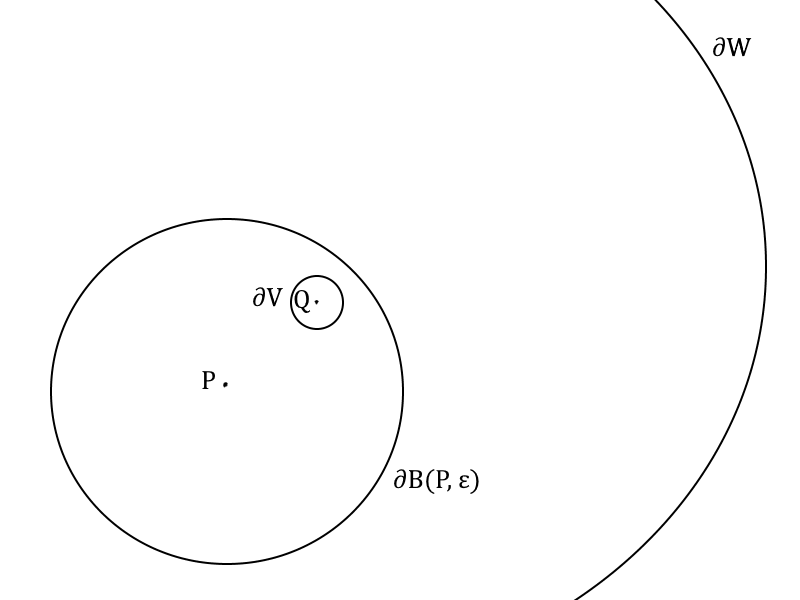
\includegraphics[width=\linewidth]{estimating_scales.png}
\end{subfigure}
\begin{subfigure}[b]{0.4\linewidth}
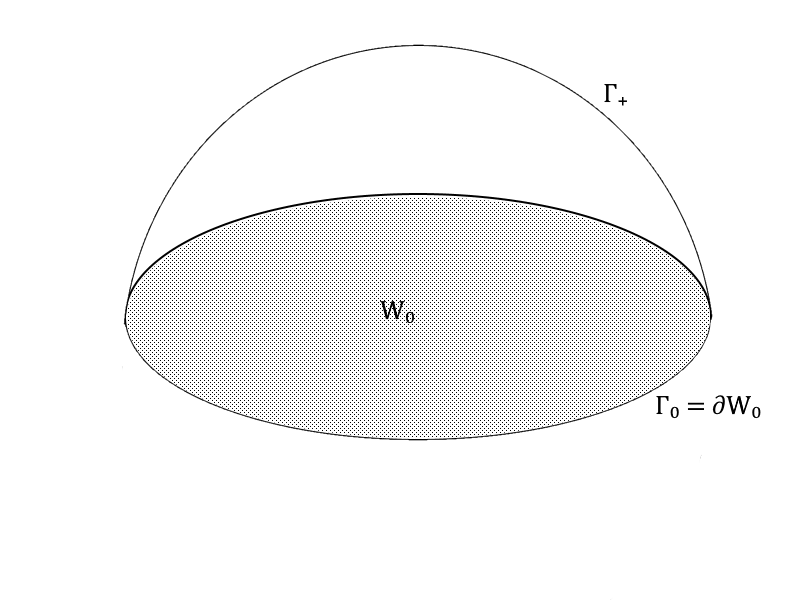
\includegraphics[width=\linewidth]{estimate homotopy.png}
\end{subfigure}
\caption{An illustration of the proof of Lemma \ref{mollifier sublemma}. On the left, the relative scales of balls involved in the proof of the lemma for $\gamma \ll 1$: $V$ is much smaller than $B_\varepsilon$, which in turn is tiny compared to $W$. On the right, $\Gamma_+$ and $W_0$ have the same homology class and the same boundary $\Gamma_0$, and $W_0$ is a slight deformation of a small ball in $\RR^{d - 1}$, so an integral $\int_{\Gamma_+} \omega$ can be approximated by the integral of $\star_{W_0} \omega$ over a small ball.}
\label{estimating figures}
\end{figure}

\begin{proof}
TODO: Update this proof We first claim that for $r > 0$ so small that $B(Q, 2r) \subseteq B_\varepsilon$,
\begin{equation}\label{bound the kernel}
\sup_{y \in B(Q, 2r)} \chi_\varepsilon(x - y) \lesssim \inf_{y \in B(Q, r)} \chi_\varepsilon(x - y).
\end{equation}
In the euclidean case (with constant equal to $4$) this result can be isolated from the proof of \cite[Theorem 7.3]{Giusti77}.
Otherwise, we can use the smallness of $\varepsilon$ and the Taylor expansion of the metric to approximate $g$-balls by euclidean balls.
This suffices to prove (\ref{bound the kernel}), since $\chi_\varepsilon$ is uniformly continuous.

Now let $V := B(Q, 2\delta\varepsilon)$.
Integrating (\ref{bound the kernel}) against $1_V(|\psi| \cdot |\dif u| - \star(\dif u \wedge \psi))$,
\begin{equation}\label{kernel bounded}
(1_V(|\psi| \cdot |\dif u| - \star(\dif u \wedge \psi)))_\varepsilon(x) \lesssim \inf_{y \in B(Q, \delta\varepsilon)} \chi_\varepsilon(x - y) \int_V \star |\psi| \cdot |\dif u| - \dif u \wedge \psi.
\end{equation}
To estimate the right-hand side of (\ref{kernel bounded}) we introduce a new coordinate system $(\tilde x^\mu)$ of normal coordinates based at $Q$ which are \dfn{compatible} with $(x^\mu)$ in the sense that $\dif \tilde x^0(Q)$ is a scalar multiple of $\dif x^0(Q)$.
We write $\tilde g$ for the metric written in these new coordinates, and write $\tilde \psi$ for their vertical $d-1$-form.
By compatibility, $\tilde \psi = \psi + O(\varepsilon)$, so
\begin{equation}\label{split up T Ttilde}
\int_V \star |\psi| \cdot |\dif u| - \dif u \wedge \psi \leq \int_V \star |\psi| \cdot |\dif u| - \dif u \wedge \tilde \psi + O(\varepsilon) \int_V \star |\dif u|.
\end{equation}
The error term here is given by Corollary \ref{doubling dimension} and the assumption $\rho \lesssim 1$ as $\lesssim \gamma^2 \int_{B(Q, \delta\varepsilon)} \star |\dif u|$.
To estimate the dominant term in (\ref{split up T Ttilde}) we assume that $\gamma$ is chosen so small that $\sigma > 2\delta\varepsilon$, so that if we set $W := B(Q, \sigma)$ and apply the monotonicity formula and compatibility to obtain $A \geq 0$ such that
\begin{align*}
(2\delta\varepsilon)^{1 - d} &\int_V \star |\psi| \cdot |\dif u| - \dif u \wedge \psi \\
&\leq \sigma^{1 - d}\int_W \star |\dif u| + (2\delta\varepsilon)^{1 - d} \int_V \star(|\psi| - 1)|\dif u| + 2A\sigma^{3 - d} \int_W \star |\dif u| - (2\delta\varepsilon)^{1 - d}\int_V \dif u \wedge \psi\\
&\leq \sigma^{1 - d}\int_W \star |\dif u| - \dif u \wedge \psi + (2\delta\varepsilon)^{1 - d} \int_V \star(|\psi| - 1)|\dif u| + 2A\sigma^{3 - d} \int_W \star |\dif u| \\
&\qquad + O(\varepsilon \sigma^{1 - d}) \int_W \star |\dif u| + \sigma^{1 - d}\int_W \dif u \wedge \tilde \psi - (2\delta\varepsilon)^{1 - d}\int_V \dif u \wedge \tilde \psi\\
&=: I_1 + I_2 + I_3 + I_4 + I_5 - I_6.
\end{align*}
We apply (\ref{hypothesis on mollifier sublemma}) to bound $I_1 \leq \gamma^{1/2}$, and we use the Taylor expansion of the metric on $V$ to bound $|\psi| - 1 \lesssim \varepsilon^2$ on $B_\varepsilon$.
By Corollary \ref{doubling dimension} and the assumption $\rho \lesssim 1$, it follows that $I_2 + I_3 + I_4 \lesssim \gamma^{1/(d - 1)}$.

To estimate $I_5 - I_6$, we apply the monotonicity formula and compatibility again:
\begin{align*}
I_5 - I_6 &\lesssim \sqrt{1 + (d - 1) \log \frac{\sigma}{2\delta\varepsilon}} \sqrt{\sigma^{1 - d} \int_W \star |\dif u|} \sqrt{\int_{2\delta\varepsilon}^\sigma \partial_r \left[e^{Ar^2} r^{1 - d} \int_{B(Q, r)} \star |\dif u|\right] \dif r}\\
&\qquad + \varepsilon \sigma^{1 - d} \int_W \star |\dif u| + \varepsilon (2\delta\varepsilon)^{1 - d} \int_V \star |\dif u| \\
&=: J_1 J_2 J_3 + J_4 + J_5.
\end{align*}
We have $J_1 \lesssim -\log \gamma$, from Corollary \ref{doubling dimension} we have $J_2 \lesssim 1$, and finally $J_4 + J_5 \lesssim \gamma^4$.
So, we need to get a gain from $J_3$, which we do as follows:
\begin{align*}
J_3^2 &\leq \sigma^{1 - d} \int_W \star |\dif u| - (2 \delta \varepsilon)^{1 - d} \int_V \star |\dif u| + 2A\sigma^{3 - d} \int_W \star |\dif u| \\
&= \sigma^{1 - d} \int_W \star |\dif u| - \dif u \wedge \psi + \sigma^{1 - d} \int_W \dif u \wedge (\psi - \tilde \psi) + \sigma^{1 - d} \int_W \dif u \wedge \tilde \psi \\
&\qquad - (2 \delta\varepsilon)^{1 - d} \int_V \star |\dif u| + 2A \sigma^{3 - d} \int_W \star |\dif u| \\
&=: K_1 + K_2 + K_3 - K_4 + K_5.
\end{align*}
Then $K_1 = I_1 \leq \gamma^{1/2}$, $K_2 \lesssim I_3 \lesssim \gamma^4$, and $K_5 = I_2 \lesssim \gamma^{1/(d - 1)}$.

To estimate $K_3 - K_4$ we observe that for $u = 1_U$,
\begin{equation}\label{K3 calculus}
K_3 = \sigma^{1 - d} \int_W \dif u \wedge \tilde \psi = \sigma^{1 - d} \int_{U \cap \partial W} \tilde \psi.
\end{equation}
We decompose
$$\partial W = \Gamma_+ \cup \Gamma_0 \cup \Gamma_-$$
where $\tilde x^0 > 0$ on $\Gamma_+$ and $\tilde x^0 < 0$ on $\Gamma_-$. Then all positive contributions to the integral in the right-hand side of (\ref{K3 calculus}) come from $\Gamma_+$.
Moreover, as $d-1$-cells in $M$, $\partial \Gamma_+ = \Gamma_0$, but also if we set $N = \{\tilde x^0 = 0\}$ and $W_0 = W \cap N$, then $\Gamma_0 = \partial W_0$.
In particular, there is a homotopy relating $\Gamma_+$ and $\partial W_0$ which holds $\Gamma_0$ fixed.
Since $\dif \psi = 0$, we can use (\ref{partial Br is a variety}) as follows:
\begin{align*}
K_3 &\leq \sigma^{1 - d} \int_{\Gamma_+} \tilde \psi = \sigma^{1 - d} \int_{W_0} \tilde \psi \leq |\Ball^{d - 1}| + O(\sigma^2).
\end{align*}
Hence by Corollary \ref{doubling dimension},
$$K_3 \leq |\Ball^{d - 1}| + O(\sigma^2) \leq K_4 e^{O(\varepsilon\delta)^2} + O(\sigma^2) \leq K_4 + O(\sigma^2) \leq K_4 + O(\gamma^{1/(d - 1)}).$$
In conclusion, $J_3 \lesssim \gamma^{\min(1/4, 1/(d - 1))}$, and hence by (\ref{kernel bounded}) we have for some $q > 0$ that
$$(1_V(|\dif u| - \star(\dif u \wedge \psi)))_\varepsilon(x) \ll (\delta\varepsilon)^{d - 1} \gamma^q \inf_{y \in B(Q, \delta\varepsilon)} \chi_\varepsilon(x - y).$$
Finally, by Corollary \ref{doubling dimension},
\begin{align*}
(\delta\varepsilon)^{d - 1} \inf_{y \in B(Q, \delta\varepsilon)} \chi_\varepsilon(x - y) &\lesssim (1_{B(Q, \delta\varepsilon)} |\dif u|)_\varepsilon(x). \qedhere
\end{align*}
\end{proof}

\begin{proof}[Proof of Lemma \ref{main mollifier lemma}]
TODO: Update this proof to use $\psi$
Let $\delta = \gamma^d > 0$.
By running a greedy algorithm, we construct a cover $\mathcal V = \{V_n: 1 \leq n \leq N\}$ of $\partial^* U \cap B_{\varepsilon(1 - 2\delta)}$ by balls of radius $2\delta\varepsilon$, centered on points $Q_n \in \partial^* U \cap B_{\varepsilon(1 - \delta)}$, which is \dfn{efficient} in the sense that the dilates $V_n/2 := B(Q_n, \delta\varepsilon)$ are disjoint.
We set $V_0 := B_\varepsilon \setminus B_{\varepsilon(1 - 2\delta)}$.

To bring the $\psi$ inside the convolution we compute
\begin{align*}
(|\psi| \cdot |\dif u|)_\varepsilon
&= \int_{B_\varepsilon} |\psi|(x - y) |\dif u|(x - y) \chi_\varepsilon(y) \dif y \\
&= \int_{B_\varepsilon} |\psi|(x) |\dif u|(x - y) \chi_\varepsilon(y) \dif y + \int_{B_\varepsilon} ||\psi|(x - y) - |\psi|(x)| \cdot |\dif u|(x - y) \chi_\varepsilon(y) \dif y
\end{align*}
and observe that $||\psi|(x - y) - |\psi|(x)| \lesssim \dist(x, y) \lesssim \varepsilon \lesssim \gamma^4$.
Since $\dif u$ is supported in $\bigcup_n V_n$, it follows that
\begin{equation}\label{sum over cover}
|\psi| \cdot |\dif \varphi| - \star(\dif \varphi \wedge \psi)
\leq O(\gamma^4) |\dif \varphi| + \sum_{n=0}^N (1_{V_n}(|\psi| \cdot |\dif u| - \star(\dif u \wedge \psi)))_\varepsilon.
\end{equation}

We claim that there exists $c > 0$ such that on $B_\sigma \cap \{c\gamma^2 < \varphi < 1 - c\gamma^2\}$,
\begin{equation}\label{V0 case}
(1_{V_0}(|\psi| \cdot |\dif u| - \star(\dif u \wedge \psi)))_\varepsilon \lesssim \gamma |\dif u|_\varepsilon.
\end{equation}
The proof of (\ref{V0 case}) is essentially given by \cite[pg92]{Giusti77}, so we just sketch it.
For $y \in V_0$, $\chi_\varepsilon(x - y) \lesssim \delta/\varepsilon^d$, so using Corollary \ref{doubling dimension}, one can show
$$\int_{V_0} \chi_\varepsilon(x - y)(|\psi| \cdot |\dif u| - \star(\dif u \wedge \psi))(y) \dif y \lesssim \frac{\gamma^d}{\varepsilon}.$$
Here we used $||\psi||_{L^\infty} \lesssim 1$.
One can use \cite[Lemma 7.1]{Giusti77}, the assumption $c\gamma^2 < \varphi < 1 - c\gamma^2$, and the fact that $g$ is a perturbation of the euclidean metric to obtain
$$\int_{B_\varepsilon} \chi_\varepsilon(x - y) |\dif u|(y) \dif y \gtrsim \frac{\gamma^{d - 1}}{\varepsilon}$$
which then implies (\ref{V0 case}).

Since $\mathcal V$ is efficient, we can sum (\ref{V0 case}) and Lemma \ref{mollifier sublemma} over $n$ in (\ref{sum over cover}) to show that (\ref{claim on main mollifier lemma}) holds.
In particular near $\varphi^{-1}(y) \cap B_{\rho - 2\sigma}$, where $y \in (c\gamma^2, 1 - c\gamma^2)$, one has $|\dif u| > 0$.
Therefore $u$ is a $C^1$ submersion by \cite[Lemma 7.1]{Giusti77}, which completes the proof.
\end{proof}

\begin{lemma}\label{single mollify}
For every $\varepsilon > 0$ there exists $\delta = \delta(d, K, \varepsilon) > 0$ and $r = r(d, K, \varepsilon) > 0$ such that for any ball $B(P, \rho)$ such that $\rho < r$ and any set $U$ of least perimeter in $B(P, \rho)$ such that
$$\Exc_\rho (U, P) \leq \delta \rho^{d - 1},$$
there exists a set $V$ of $C^1$ perimeter in $B(P, (1 - \varepsilon)\rho)$ such that
\begin{align}
\star((\Phi^P)^* \normal_V \wedge \psi) &\geq (1 - o(\varepsilon^2))|\psi|, \label{single mollify normal}\\
|\partial V \cap B(P, (1 - \varepsilon)\rho)| &\leq \eta(V, B(P, (1 - \varepsilon)\rho)) + \varepsilon \Exc_\rho (U, P), \label{single mollify minimality}
\end{align}
and for $0 < \varpi \leq (1 - \varepsilon)\rho$,
\begin{equation}
|\Exc_\varpi (U, P) - \Exc_\varpi (V, P)| \leq \varepsilon \Exc_\rho (U, P) + C|K| \rho^{d + 1}. \label{single mollify excess}
\end{equation}
\end{lemma}
\begin{proof}
If not, then there exist balls $B_n := B(P_n, \rho_n)$ and sets $U_n$ of least perimeter in $B_n$ such that
\begin{equation}\label{single mollify Excess assumption}
\Exc_{\rho_n} (U_n, P_n) \leq n^{-2} \rho_n^{d - 1},
\end{equation}
and $\rho_n \leq 1/n$, but such that for every set $V_n$ of $C^1$ perimeter in $B(P_n, (1 - \varepsilon) \rho_n)$, at least one of (\ref{single mollify normal}), (\ref{single mollify minimality}), or (\ref{single mollify excess}) fail.
Applying an isometry, we may assume that $P_n = O$ and
\begin{equation}\label{excess is the s3 integral}
\Exc_{\rho_n} (U_n, O) = \int_{B_n} \star |\psi| \cdot |\dif 1_{U_n}| - \dif 1_{U_n} \wedge \psi + O(|K| \rho_n^{d + 1}).
\end{equation}
In fact, we can assume that $\normal_{U_n}(O, \rho_n)$ is orthogonal to $\dif x^i(O)$ for all $i \geq 1$ from which it follows that
$$\int_{B_n} \partial_\mu 1_{U_n} \star 1 \dif x^\mu(O) = \int_{B_n} \partial_0 1_{U_n} \star 1 \dif x^0(O)$$
and then we can use the fact that
\begin{align*}
\star(\dif 1_{U_n} \wedge \psi) &= \star(\partial_\mu 1_{U_n} \wedge \dif x^1 \wedge \cdots \wedge \dif x^{d - 1}) = \star (\partial_0 1_{U_n} \dif x^0 \wedge \cdots \wedge \dif x^{d - 1}) \\
&= \frac{\partial_0 1_{U_n}}{\sqrt{\det g}} \star 1
\end{align*}
and the Taylor expansion of $g$ and Corollary \ref{doubling dimension} to conclude (\ref{excess is the s3 integral}).
Thus by (\ref{single mollify Excess assumption}),
\begin{equation}\label{excess vs special sequence}
\gamma_n := \rho_n^{1 - d} \int_{B(P, \rho_n)} \star |\psi| \cdot |\dif 1_{U_n}| - \dif 1_{U_n} \wedge \psi = \rho_n^{1 - d} \Exc_{\rho_n}(U, P) + |K| \rho^2 \lesssim n^{-2}
\end{equation}
is a sequence in $\ell^1$.

Now let $w_n := (u_n)_{\rho_n \gamma_n^4}$ be the mollification of $u_n$, draw $t \in [0, 1]$ uniformly at random, and let $c, q > 0$ be as in Proposition \ref{main mollifier lemma}, $a_n := c\gamma_n^2$, $b_n := 1 - c\gamma_n^2$.
By the coarea formula, Proposition \ref{Coarea2},
$$\int_{tB_n} \star |\dif w_n| = \int_0^1 |\partial^* \{w_n > y\} \cap tB_n| \dif y \geq \int_{a_n}^{b_n} |\partial^* \{w_n > y\} \cap tB_n| \dif y,$$
so by the mean value theorem, there exists $y_n \in (a_n, b_n)$ such that
$$|\partial^* \{w_n > y_n\} \cap tB_n| \leq \frac{1}{b_n - a_n} \int_{tB_n} \star |\dif w_n|.$$
We then set $V_n := \{w_n > y_n\}$, $v_n := 1_{V_n}$, so $V_n$ has $C^1$ boundary in $tB_n$, and by the above computation,
\begin{equation}\label{MVT mollifier}
|V_n \cap tB_n| \leq \frac{1}{1 - 2c\gamma_n^2} \int_{tB_n} \star |\dif w_n|.
\end{equation}
Since $\grad w_n$ is normal to the level sets of $w_n$, $\normal_{V_n} = \dif w_n/|\dif w_n|$.
So by (\ref{claim on main mollifier lemma}),
$$\star(\normal_{V_n} \wedge \psi) \geq |\psi| \cdot (1 - o(\gamma_n^q)).$$
Thus for $n$ large, $V_n$ satisfies (\ref{single mollify normal}).

Arguing completely analogously to the proofs of \cite[(7.23), (7.22)]{Giusti77}, respectively, we see that
for $s \in (0, t]$ drawn uniformly at random and $\Gamma_n := \partial(sB_n)$, we have almost surely that
\begin{align}
||u_n - v_n||_{L^1(\Gamma_n)} &\ll \rho_n^{d - 1} \gamma_n \label{trace of vn} \\
|\partial V_n \cap sB_n| &\leq |\partial^* U_n \cap sB_n| + o(\rho_n^{d - 1} \gamma_n). \label{difference of surface area}
\end{align}
It is crucial that $(\gamma_n) \in \ell^1$ in order to be able to prove that.

For $s = t$, the estimate
\begin{equation}
||\partial^* U_n \cap tB_n| - |\partial V_n \cap tB_n|| \ll \gamma_n \rho_n^{d - 1} \label{mollifier quant2}
\end{equation}
is the conjunction of (\ref{trace of vn}), (\ref{difference of surface area}), and (\ref{a priori estimate 1}).
Then (\ref{single mollify minimality}) is the conjunction of (\ref{mollifier quant2}), (\ref{a priori estimate 1}), the fact that $U_n$ has least perimeter, (\ref{excess vs special sequence}) and (\ref{trace of vn}).

To derive a contradiction, we must show that $(V_n)$ satisfies (\ref{single mollify excess}) for $n$ large.
By (\ref{excess vs special sequence}) it suffices to show that for every $d-1$-form $\omega_n$,
\begin{equation}\label{mollifier quant3}
\left|\int_{sB_n} \dif(1_{U_n} - 1_{V_n}) \wedge \omega_n\right| \ll \gamma_n \rho_n^{d - 1} ||\omega_n||_{C^1}.
\end{equation}
Indeed, if this is true, then in particular it holds for $\omega_n = \dif x^\mu_n$, but then $\int_{sB_n} \dif(1_{U_n} - 1_{V_n}) \wedge \omega_n$ is the $\mu$th term in the negative part of the excess.

Integrating by parts,
$$\left|\int_{sB_n} \dif (u_n - v_n) \wedge \omega_n\right| \leq ||\omega_n||_{L^\infty} ||u_n - v_n||_{L^1(\Gamma_n)} + ||\dif \omega_n||_{L^\infty} \int_0^t ||u_n - v_n||_{L^1(\partial(sB_n))} \dif s.$$
By (\ref{trace of vn}),
$$\limsup_{n \to \infty} ||\omega_n||_{C^1}^{-1} \gamma_n^{-1} \rho_n^{1 - d} \left|\int_{sB_n} \dif(u_n - v_n) \wedge \omega_n\right| \leq \limsup_{n \to \infty} \int_0^s \gamma_n^{-1} \rho_n^{1 - d} ||u_n - v_n||_{L^1(\partial(rB_n))} \dif r.$$
Moreover, (\ref{trace of vn}) holds with $s$ replaced by almost any $r$, so
$$f_n(r) := \gamma_n^{-1} \rho_n^{1 - d} ||u_n - v_n||_{L^1(\partial(rB_n))}$$
satisfies $(f_n) \in \ell^\infty([0, 1] \to L^\infty)$, and $f_n \to 0$ almost everywhere.
So by Fatou's lemma,
\begin{align*}
0 \leq \limsup_{n \to \infty} ||\omega_n||_{C^1}^{-1} \gamma_n^{-1} \rho_n^{1 - d} \left|\int_{tB_n} \dif(u_n - v_n) \wedge \omega_n\right| &\leq \int_0^t \lim_{n \to \infty} f_n(r) \dif r = 0. \qedhere
\end{align*}
\end{proof}

\begin{proof}[Proof of the de Giorgi lemma]
Let $c_0$ be small enough to meet the hypotheses of Lemma \ref{Miranda43} and satisfy $c_0 \leq 2^{-(d + 2)}/(A + 3)$ where $A$ is the implied constant in the $O(c_0)$ in (\ref{Miranda44 concl}).
Let $\alpha := 1/(2(1 - c_0))$, and let $V$ be the set obtained from Lemma \ref{single mollify} with $\varepsilon := c_1 < c_0$ and $c := \delta(\varepsilon)$.
By (\ref{single mollify excess}) and (\ref{approximate monotone}), for $\beta := \Exc_{B(P, \rho)} U$,
\begin{align*}
\Exc_{(1 - c_0) \rho} (V, P) &\leq \Exc_{(1 - c_0) \rho} (U, P) + c_0 \Exc_\rho (U, P) + C|K| \rho^{d + 1} \leq (1 + c_0) \Exc_\rho (U, P) + C |K| \rho^{d + 1} \\
&\leq (1 + c_0) \beta + C |K| \rho^{d + 1} =: \beta'.
\end{align*}
So by Lemma \ref{Miranda44} and our choice of $\alpha$,
\begin{align*}
\Exc_{\rho/2} (V, P) &\leq (2^{-(d + 1)} (1 - c_0)^{-(d + 1)} + Ac_0) \beta' + C |K| \rho^{d + 1} \\
&\leq (2^{-(d + 1)} + (A + 1) c_0) \beta + C |K| \rho^{d + 1}.
\end{align*}
Applying (\ref{single mollify excess}) again, we obtain $\Exc_{\rho/2} (U, P) \leq (2^{-(d + 1)} + (A + 3) c_0) \beta + C |K| \rho^{d +1}$ which implies (\ref{dGL concl}).
\end{proof}



%%%%%%%%%%%%%%%%%%%%%%%%%%%%%%%%%%%%
\section{Application to minimal laminations}\label{GornySec}
\subsection{Topological preliminaries} \label{LamPrelim}
In this section we prove our main Theorems \ref{main thm} and \ref{Gorny regularity}, somewhat simultaneously.
Throughout, we fix an oriented manifold $M$ of constant sectional curvature and dimension $2 \leq d \leq 7$.

We have a Liouville theorem in the sense that there are no global functions of least gradient on a closed hyperbolic manifold except constants.
However, the least-gradient functional is preserved by addition of constants, so we can talk about sections of flat affine line bundles with structure group $\RR = (\RR, +)$ which are locally functions of least gradient.
This approach is also taken by \cite[\S2.1]{daskalopoulos2020transverse}, which identify such bundles with representations of $\pi_1(M)$, as follows:

\begin{definition}
Let $\alpha: \pi_1(M) \to \RR$ be a representation and let $\tilde M \to M$ be the universal cover.
The \dfn{twisted product} $M \times_\alpha \RR$ is the affine line bundle whose sections are canonically identified with functions $\tilde f: \tilde M \to \RR$ such that for $\gamma \in \pi_1(M)$ and $\tilde x \in \tilde M$,
$$\tilde f(\gamma \tilde x) = \tilde f(\tilde x) + \alpha(\gamma).$$
\end{definition}

It follows that $M \times_\alpha \RR$ is flat, with structure group $\RR$.
This construction is primarily useful when $\tilde M$ is not compact, as then the maximum principle does not obstruct the existence of nontrivial solutions of elliptic PDE on $\tilde M$.
For example it applies to any complete hyperbolic manifold $M = \Hyp^d/\pi_1(M)$.

By \cite{Ruelle75}, a Ruelle-Sullivan current $T_\mu$ is a closed $d-1$-current, which is well-defined in that it does not depend on the choice of partition of unity, and hence defines a cohomology class in $H^1(M, \RR)$. So by the Hurecwiz theorem, we obtain a representation $\alpha: \pi_1(M) \to \RR$.
The construction of \cite[Theorem 8.3]{daskalopoulos2020transverse} shows that there is a section $u \in BV_\loc(M, M \times_\alpha \RR)$ such that $\dif u = T_\mu$.

TODO: Do I care about orientation bundles?

TODO: Exposit and clean this up

\begin{proposition}\label{existence of jump graphs}
Let $u \in BV(M)$ be not essentially discontinuous.
Assume that $J_u$ is an embedded hypersurface and the traces of $u$ along each component $N$ of $J_u$ are constant on each side of $N$.
Then there exists an affine line bundle $E \to M$, which is flat with structure group $\RR$, and a section $Ju: M \to E$ such that $Ju$ is locally constant on $M \setminus \lambda$ and for each leaf $N$ of $\lambda$, the amounts that $u, Ju$ jump along $N$ are equal.
\end{proposition}
\begin{proof}
We first observe that $\pi_0(M \setminus \lambda)$ is nonempty and countable, since $\lambda$ is a countable union of null sets and so $M \setminus \lambda$ is nonempty, and since $\lambda$ only has countably many connected components.
We define a new lamination $\tilde \lambda$, as follows. Initialize $\tilde \lambda := \lambda$ and replace each leaf in $\lambda$ with its connected components.
We then adjoin further leaves to $\tilde \lambda$ so that for each $U \in \pi_0(M \setminus \tilde \lambda)$, if $\mathcal V(U)$ denotes the set of components which are adjacent to $U$, then $\overline{U \cup \bigcup_{V \in \mathcal V(U)} V}$ is contained in a simply connected subset of $M$.

We set $\{U_i: i \in I\} = \pi_0(M \setminus \tilde \lambda)$ for a countable set $I$.
We endow $I$ with the structure of a weighted directed multigraph, where the set of edges $E_{ij}$ from $i$ to $j$ is $E_{ij} := \pi_0(\partial U_i \cap \partial U_j)$ if $i \neq j$.
Thus each element of $E_{ij}$ is a leaf of $\tilde \lambda$.
We weight an edge $N \in E_{ij}$ by the amount that $u$ jumps along any curve $\gamma$ from $U_i$ to $U_j$ transverse to $N$ when $\gamma$ passes through $N$.
The leaves we adjoined all have weight $0$.

We choose $x_i \in U_i$ for each $i \in I$.
We call a path $\sum_k N_k$ through $I$, where $N_k$ is an edge $i_k \to j_k$, a \dfn{boundary} if there are curves $\gamma_1, \dots, \gamma_m$, where $\gamma_k$ is a curve $x_{i_k} \to x_{j_k}$ that is transverse to $\tilde \lambda$ and passes through $N_k$ exactly once, and the homology class $[\sum_k \gamma_k]$ is zero.
We call a path a \dfn{cycle} if its total weight is $0$, and two paths \dfn{homologous} if their difference is a boundary.

\begin{claim}
Every boundary is a cycle.
\end{claim}
\begin{proof}[Proof of claim]
Let $k = 1, \dots, n$, let $\gamma := \sum_k \gamma_k$ be the associated $1$-chain to a boundary $\sum_k N_k$, and let $w_k$ be the weight of $N_k$.
If we set $v$ to be $u$ on $U_{i_1}$, $u - w_1$ on $U_{i_2}$, etc., $u - \sum_{k < n} w_k$ on $U_{i_n}$, then $v$ is continuous away from $N_{i_n}$ where it has a jump discontinuity of size $\sum_k w_k$.
Then $\int_\gamma \dif v = 0$ but also $\int_\gamma \dif v = \sum_k w_k$.
\end{proof}

Let $P_{ij}$ be the set of paths $i \to j$, thus if $p, q \in P_{ij}$ are homologous, then $p - q$ is a cycle.
On the other hand, if $i, j$ are adjacent, then for $N, N' \in E_{ij}$ and $\gamma, \gamma': x_i \to x_j$ which are respectively transverse to $N, N'$ and do not leave $\overline U_i \cup \overline U_j$, $[\gamma - \gamma'] = 0$, so $N, N'$ are homologous and hence $N - N'$ is a cycle.

We now define $V_i$ to be the interior of $\overline U_i \cup \bigcup_{E_{ij} \neq \emptyset} \overline U_j$.
Then $(V_i)$ is an open cover of $M$.
For $x \in V_i \setminus \tilde \lambda$, let $j(x)$ be such that $x \in U_{j(x)}$, and let $Ju_i(x)$ be the weight of some (and hence any) edge in $E_{ij(x)}$ if $j(x) \neq i$, or $Ju_i(x) = 0$ if $j(x) = i$.
Then $Ju_i$ is well-defined, locally constant, and jumps by the same amount along each leaf of $\tilde \lambda$ in $V_i$ as $u$.
Moreover, on $V_i \cap V_j$, $Ju_i - Ju_j = Ju_i(x_j)$ which is constant.
Now the desired bundle $E$ exists with flat trivializations $V_i$ and transition functions $s_{ij} := Ju_i(x_j)$.
If $V_i \cap V_j \cap V_k$ is nonempty, then it is contained in a simply connected set and so $s_{ik} = s_{ij} + s_{jk}$.
\end{proof}

\begin{figure}
\centering
\begin{subfigure}[b]{0.4\linewidth}
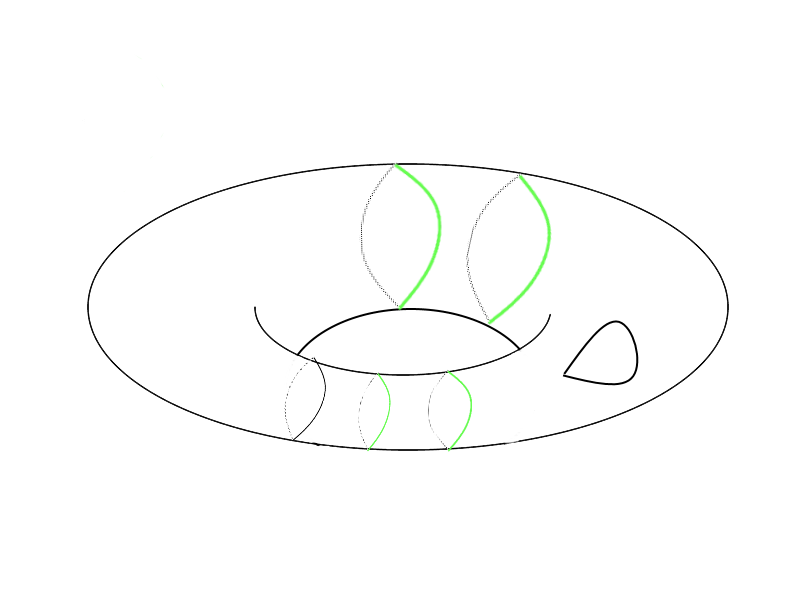
\includegraphics[width=\linewidth]{sample torus.png}
\end{subfigure}
\begin{subfigure}[b]{0.4\linewidth}
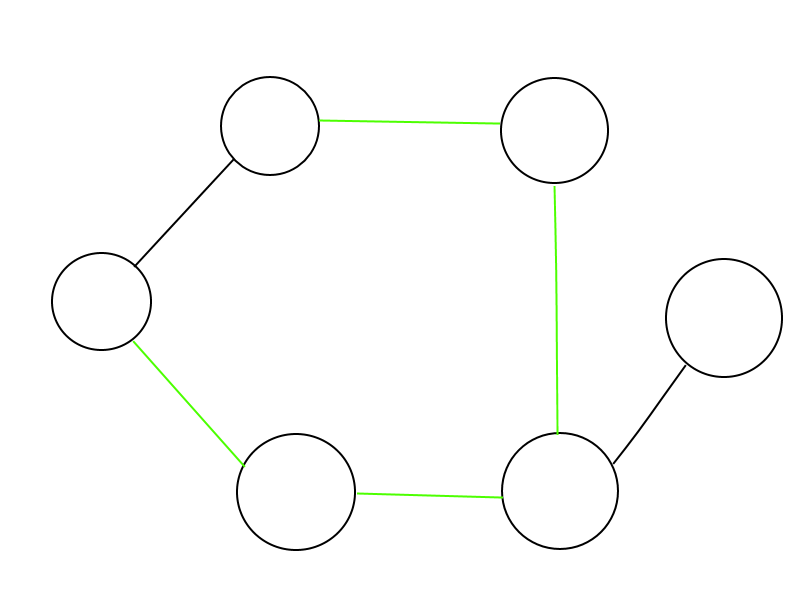
\includegraphics[width=\linewidth]{torus graph.png}
\end{subfigure}
\caption{The proof of Proposition \ref{existence of jump graphs} in case $M = \mathbf T^2$ and $u$ has two jump discontinuities, along each of the black loops. Note that we have to adjoin green leaves in order to ensure the simple connectedness condition, and that if we were to retract the green edges of the graph, then there would be a vertex of $I$ with a self-loop.}
\label{torus graphs}
\end{figure}
%%%%%%%%%%%%%%%%%%%%%%%%%%%%%%%%%%%%%%%%%%%%%%%%%

\subsection{Regularity of functions of least gradient}
In order to apply Proposition \ref{construction of minimal partitions}, it will be convenient to reduce to the cases that a given function $u$ of least gradient is either continuous, or the jump function of a lamination whose moduli space of leaves is discrete.
This will be possible if we prove Theorem \ref{Gorny regularity}, and thanks to Proposition \ref{construction of minimal partitions} this can be done.

\begin{lemma}
Let $u$ be a function of least gradient and $x \in M$. Then either the germ of $u$ at $x$ is continuous, or there exists a level set $N$ of $u$ such that $x \in N$ and the traces of $u$ along $N$ are constant and nonequal.
\end{lemma}
\begin{proof}
Reasoning identically to the proof of \cite[Proposition 3.9]{górny2017planar} (TODO Clarify this point) we see that $u$ jumps at $x$ iff
$$\inf\left\{t \in \RR: \lim_{r \to 0} \frac{|\{u \leq t\} \cap B(x, r)|}{|B(x, r)|} = 1\right\} \neq \sup\left\{t \in \RR: \lim_{r \to 0} \frac{|\{u \geq t\} \cap B(x, r)|}{|B(x, r)|} = 1\right\}.$$
The claim now follows from \cite[Theorem 4.1]{HakkarainenKorteLahtiShanmugalingam+2015}, which is true for functions of least gradient on metric measure spaces and in particular holds in our setting.
\end{proof}

\begin{proof}[Proof of Theorem \ref{Gorny regularity}]
Let $u$ be a function of least gradient on $M$ with jump set $J_u$.
Combining the above propositions TODO, there exists a unique (up to isomorphism) decomposition $u = u_j - u_c$ into sections $u_j, u_c: M \to E$, where $E$ is a flat affine line bundle with structure group $\RR$, such that $u_j$ is locally constant on $M \setminus \lambda$, $u_j$ has the same jumpset, with the same traces on each leaf, as $u$, and $u_c$ has no jump discontinuties.
Reasoning identically to \cite[pg11]{górny2017planar} we see that $u_j, u_c$ have locally least gradient.
Repeating the reasoning from the start of this proof and using the fact that $u_c$ has no jump discontinuities, it follows that $u_c$ is continuous.
\end{proof}

%%%%%%%%%%%%%%%%%%%%%%%%%%%%%%%%%%%%%%%

\subsection{Functions of least gradient induce minimal laminations}

\begin{definition}
A \dfn{minimal partition} is a closed set $\lambda$ which has been partitioned into (disjoint, embedded, without boundary) minimal hypersurfaces, called the \dfn{leaves} of $\lambda$.
\end{definition}

\begin{proposition}\label{construction of minimal partitions}
Let $u$ be a set of least gradient on $M$, $2 \leq d \leq 7$.
Then the connected components of the level sets $\partial \{u > y\}$ of $u$ define a minimal partition with support $\supp \dif u$, and each level set only has locally finitely many connected components, each of which is stable.
\end{proposition}
\begin{proof}
Let $\mathscr P$ be the set of all connected components of all level sets of $u$.
By \cite[Theorem 1]{BOMBIERI1969}, for every $y \in \RR$, $\{u > y\}$ has least perimeter.
The argument of \cite{BOMBIERI1969} only relies on the coarea formula and Miranda stability theorem, which we proved for manifolds in \S\ref{Prelims}, so it applies in our setting.
So by Theorem \ref{main thm}, $\{u > y\}$ is bounded by connected, embedded, stable minimal hypersurfaces; in particular, the elements of $\mathscr P$ are connected, embedded, stable minimal hypersurfaces.
Moreover, the decomposition of $\partial \{u > y\}$ into components is locally finite.
Indeed, by Corollary \ref{doubling dimension}, each connected component $N$ of $\partial \{u > y\}$ satisfies $|N \cap B| \gtrsim r^{d - 1}$, yet $\partial \{u > y\}$ has locally finite perimeter, thus $|\partial \{u > y\} \cap B| < \infty$.

We now show that any two distinct $N_1, N_2 \in \mathscr P$ are disjoint.
If $x \in N_1 \cap N_2$, then let $N_i$ be a component of $\partial \{u > y_i\}$.
Without loss of generality, $y_1 \leq y_2$, thus $\{u > y_2\} \subseteq \{u > y_1\}$, and hence $N_2 \subseteq \overline{\{u > y_1\}}$.
In particular $N_2$ lies on one side of $N_1$, so by the maximum principle, the germs of $N_1$ and $N_2$ at $x$ are identical.
So by unique continuation, $N_1 = N_2$.

The following statements are manifestly equivalent:
\begin{enumerate}
\item $x \notin \supp \dif u$.
\item The germ of $u$ at $x$ is constant.
\item If $u > y$ on one side of some hypersurface that passes through $x$, then $u > y$ near $x$.
\item $x \notin \partial \{u > y\}$ for any $y$.
\item $x \notin N$ for any leaf $N$ associated to $u$.
\end{enumerate}
It follows that $\supp \dif u$ is the support of the minimal partition whose set of leaves is $\mathscr P$.
\end{proof}

It is instructive to observe that the seemingly purely set-theoretic claims of the previous proposition require Theorem \ref{main lma}.
Indeed, in case $d = 8$, we could define for $x \in \RR^4$, $y \in \RR^3$, $z \in \RR$,
$$u(x, y, z) = \begin{cases}
-1, & z < 0 \\
0, & z > 0, |x|^2 < |y|^2 + z^2 \\
1, & z > 0, |x|^2 > |y|^2 + z^2
\end{cases}$$
and then the level sets of $u$ are the Simons cone $\{|x|^2 = |y|^2 + z^2\} \cap \{z \geq 0\}$ and the hyperplane $\{z = 0\}$, which intersect at $0$ and are minimal, thus $u$ has least gradient on $\RR^8$.

\begin{proof}[Proof of Theorem \ref{main thm}]
Let $u$ be a function of least gradient.
By Proposition \ref{construction of minimal partitions}, $\supp \dif u$ is the support of a minimal partition $\lambda$ whose leaves are the level sets of $u$, where each level set is the locally finite union of its components, and so by \cite[TODO]{BackusCML} $\lambda$ is a minimal lamination.

Let $(y_i, x_i): U_i \to Y_i \times N_i$, $i \in I$, be an atlas for $\lambda$.
Here $K_i \subseteq Y_i$ is the moduli space of leaves of $\lambda$ in $Y_i$.
Then, on the fibers $N_{y_i} := \{y_i\} \times N_i$, $u$ is constant.
Indeed, either $y_i \in K_i$ and so $N_{y_i}$ is contained in a level set of $u$, or $y_i \notin K_i$, so $N_{y_i}$ lies in a \dfn{plaque}, or component of $M \setminus \supp \lambda$, and hence $\dif u = 0$ in an open neighborhood of $N_{y_i}$.

In particular, we can define $u_i: Y_i \to \RR$ by setting $u_i(y_i) = u(y_i, x_i)$ for any $x_i \in N_i$.
Then $u_i$ satisfies the maximum principle: there do not exist $y_{i,1}$ and $y_{i,2}$ such that $u_i'(y_{i,1}) > 0$ and $u_i'(y_{i,2}) < 0$.
If there do, then we can replace $u$ with a competitor $\tilde u$ on $U_i$ by setting $\tilde u$ to be $u$ away from the region $\{y_{i,1} < y_i < y_{i,2}\}$ and to be constant on that region; then $\int_{U_i} \star |\dif \tilde u| < \int_{U_i} \star |\dif u|$ which contradicts that $u$ has least gradient.
So $u_i$ is either nondecreasing or nonincreasing on $Y_i$; if it is nonincreasing, we replace $y_i$ with $-y_i$.
With this convention, for any partition of unity $(\chi_i)$,
$$\normal^\sharp := \sum_{i \in I} \chi_i \frac{\grad y_i}{|\grad y_i|}$$
is a global section of the sphere bundle $SM$ which is normal to every leaf of $\lambda$. In particular, $\normal^\sharp$ defines an orientation $[\normal^\sharp]$ of $\lambda$.

We now define a transverse measure $\mu$ to $\lambda$.
First, by the G\'orny decomposition, there exist sections $u_j, u_c$ of locally least gradient such that $u_j$ is a jump section, $u_c$ is continuous, and $u = u_c + u_j$.
Then these define minimal laminations $\lambda_j, \lambda_c$.
Moreover, $\lambda_j$ is a \emph{discrete} lamination in that its moduli space of leaves $K_{j,i}$ in $U_i$ is a discrete set, so we can define an atomic measure $\mu_{j,i}(\{N\})$ to be the amount that $u_j$ jumps along $N$.
It is clear that the transition maps $\psi_{ik}$, $i,k \in I$, are measure-preserving.

As for the continuous part, we define a new (possibly non-Lipschitz) flow box coordinate $\tilde y_i$ by setting $\tilde y_i$ to equal $u_{c,i}$ on each leaf, and extend to the plaques by imposing that $\tilde y_i$ must be strictly increasing in $y_i$, and linear in $y_i$ on each plaque.
Then $y_i \mapsto \tilde y_i$ is a homeomorphism $Y_i \to \tilde Y_i$ for some $\tilde Y_i \subseteq \RR$, since $u_{c,i}$ is continuous and nondecreasing in $y_i$.
Here we are assuming that each flow box $U_i$ is contained in a trivialization of the affine line bundle of which $u_c$ is a section.
In particular, we may define for each Borel set $E \subset \tilde Y_i$,
$$\mu_{c,i}(E) := (\tilde y_i)_*(\star |\dif u|)(E) = \int_{(\tilde y_i)^*(E)} \star |\dif u|.$$
To see that $\psi_{ik}$ is measure-preserving we observe that $\psi_{ik}$ transforms $\tilde y_i$ to $\tilde y_k$, hence
$$\psi_{ik}^* \mu_{c,i} = \psi_{ik}^* (\tilde y_i)_* (\star |\dif u|) = (\tilde y_k)_* (\star |\dif u|) = \mu_{c,k}.$$

Summing up, $\mu_c, \mu_j$ are transverse measures and so their sum $\mu := \mu_c + \mu_j$ is also transverse.
By the disintegration theorem, for any $f \in L^1(\dif u)$,
$$\int_M f \star |\dif u| = \sum_{i \in I} \int_{K_i} \left[\int_{\{y_i\} \times N_i} \star_{y_i} \chi_i f \right] \dif \mu_i(y_i).$$
Here $\star_{y_i}$ is the Hodge star on $\{y_i\} \times N_i$ induced by $g$.
So for any $d-1$-form $\varphi$,
\begin{align*}
\int_M \dif u \wedge \varphi &= \int_M (\normal^\sharp, \varphi) \star |\dif u|
= \sum_{i \in I} \int_{K_i} \left[\int_{\{y_i\} \times N_i} \star_{y_i} \chi_i \star_{y_i} \varphi \dif \nu_{y_i}\right] \dif \mu_i(y_i) \\
&= \sum_{i \in I} \int_{K_i} \left[\int_{\{y_i\} \times N_i} \chi_i \varphi\right] \dif \mu_i(y_i)
\end{align*}
which implies that $\dif u$ is the Ruelle-Sullivan current of $(\lambda, [\normal^\sharp], \mu)$.

As for the converse, let $\lambda$ be a minimal lamination, and suppose that $\dif u$ is Ruelle-Sullivan for $\lambda$.
Then $\star |\dif u|$ is transverse to the leaves of $\lambda$, so $u$ is constant on each leaf.
Now let $U \Subset M$ and let $v \in BV_\cpt(U)$, thus $V = U \setminus \supp v$ is the intersection of an open neighborhood of $\partial U$ with $U$.
If $v$ is not identically zero, then there is a positive measure set $Y \subseteq \RR$ such that for $y \in Y$, $\partial \{u > y\} \neq \partial^* \{u + v > y\}$.
But
$$V \cap \partial \{u > y\} = V \cap \partial^* \{u + v > y\}$$
so $1_{\{u > y\}}$ and $1_{\{u + v > y\}}$ are equalized by the trace map $BV_\loc(U) \to L^1_\loc(\partial U)$.
Now $\{u > y\}$ has least perimeter in $U$, so if $|U \cap \partial \{u > y\}| = |U \cap \partial^* \{u + v > y\}|$ then $\{u + v > y\}$ has least perimeter in $U$.
Each component of $\partial \{u > y\}$ and $\partial \{u + v > y\}$ is a minimal hypersurface in $U$ with the same trace, so by unique continuation,
$$\partial \{u > y\} = \partial \{u + v > y\}.$$
But this contradicts the assumption that $y \in Y$. So for each $y \in Y$,
$$|U \cap \partial \{u > y\}| < |U \cap \partial^* \{u + v > y\}|.$$
Integrating both sides in $y$ using the coarea formula, we conclude that
\begin{align*}
\int_U \star |\dif u + \dif v| - \star |\dif u| &= \int_{-\infty}^\infty |U \cap \partial^* \{u + v > y\}| - |U \cap \partial \{u > y\}| \dif y \\
&= \int_Y |U \cap \partial^* \{u + v > y\}| - |U \cap \partial \{u > y\}| \dif y > 0,
\end{align*}
and since $v$ was an arbitrary perturbation, $u$ must have least gradient.
\end{proof}


\printbibliography

\end{document}
